\capitulo{5}{Aspectos relevantes del desarrollo del proyecto}

En este apartado se va a comentar, a manera de resumen temporal, el desarrollo del proyecto. Es en este apartado donde se comentarán las opciones y decisiones tomadas, los problemas surgidos y todos los aspectos importantes. Se ha considerado que la mejor forma de organizar este apartado es en secciones donde se comenta cada aspecto del desarrollo.

\section{Desarrollo FIS-HUBU}\label{desarrolloFH}
FIS-HUBU es un proyecto que permite realizar vídeo llamadas entre responsables y pacientes con Parkinson para realizar rehabilitaciones de manera \textit{online}, es decir, sin la necesidad de desplazarse hasta la consulta o el hospital. Este proyecto se ha financiado por la universidad Carlos III, con el proyecto  <<Fundación Burgos por la investigación de la salud complejo asistencial universitario de Burgos PI19/00670. Estudio de factibilidad y coste-efectividad del uso telemedicina con un equipo multidisciplinar para enfermedad de Parkinson>>.

Esta aplicación, que ha sido desarrollada junto con mi compañero José Luis Garrido Labrador, permite por parte del responsable observar y evaluar la evolución del estado de un paciente, esta evolución también es visible para el paciente que puede ver su propio progreso.

La aplicación puede dividirse en distintas partes que serán comentadas a continuación.
\subsection{Vídeo llamadas}
El punto principal de la aplicación, y por ende su principal uso, son las vídeo llamadas entre pacientes y responsables o terapeutas que permiten sustituir la rehabilitaciones presenciales en consulta por rehabilitaciones \textit{online}. Esto permite que se puedan dar más a menudo y puedan ser accesibles para un mayor número de personas, sobre todo para aquellos pacientes que no se pueden desplazar o viven aislados geográficamente.

Primero se realizó una investigación sobre las principales plataformas de vídeo llamadas. Lo que se estaba buscando de estas plataformas era:
\begin{itemize}
	\item Creación de llamadas de manera sencilla y automática. Si es posible a partir de \textit{url}.
	\item Vídeo llamada estable sin necesidad de una gran conexión.
	\item Plataforma que permita grabar la cámara de los pacientes.
	\item Plataforma gratuita.
\end{itemize}

Dentro de las plataformas que se investigaron están las más conocidas aplicaciones de este tipo como puede ser \textit{Skype} o \textit{Hangouts}, pero al final se decidió utilizar {\textit{Jitsi}\footnote{Jitsi: \url{https://jitsi.org/}} ya que proporciona todas las necesidades anteriormente comentadas, y además permite en un futuro poder crear un servidor propio donde poder modificar parámetros como la calidad de las llamadas.

\subsection{Responsable}
Parte de la aplicación donde los responsables pueden realizar las siguientes tareas:
\begin{itemize}
	\item Iniciar una vídeo llamada con un paciente.
	\item Evaluar la evolución de los pacientes.
	\item Modificar las evaluaciones de los pacientes.
	\item Comprobar la evolución de los pacientes.
\end{itemize}

La interfaz de la aplicación para tipo de usuario es sencilla y clara, como se puede ver en el menú principal, figura~\ref{fig:menuPaciente}, o en el menú de estadísticas, figuras~\ref{fig:menuest} y~\ref{fig:ejemploest}.

\begin{figure}[h]
	\centering
	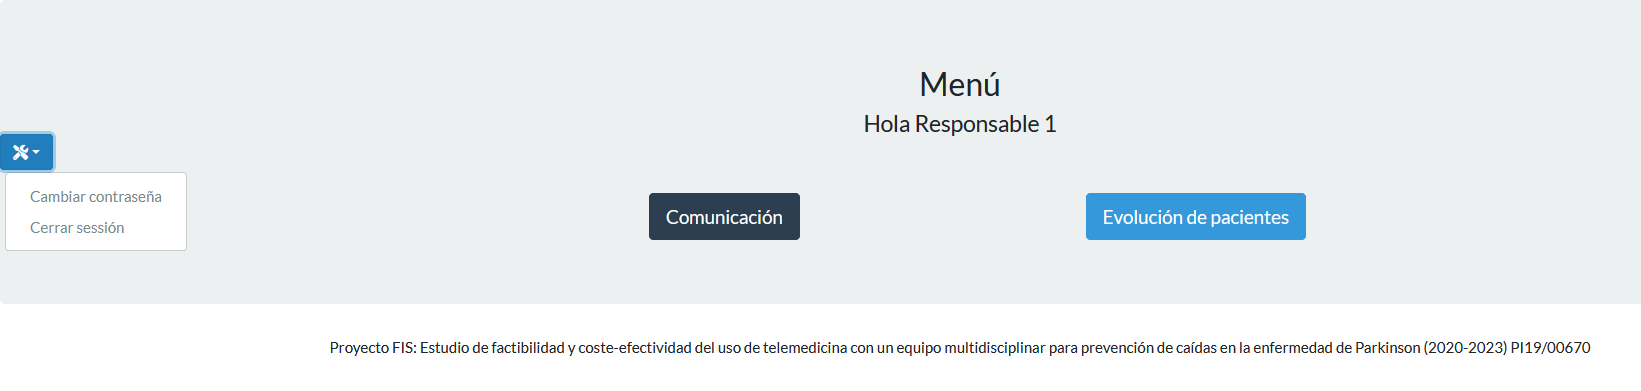
\includegraphics[width=1\textwidth]{menuResponsable}
	\caption{Menú principal de un responsable.}
	\label{fig:menuPaciente}
\end{figure}

\begin{figure}[h]
	\centering
	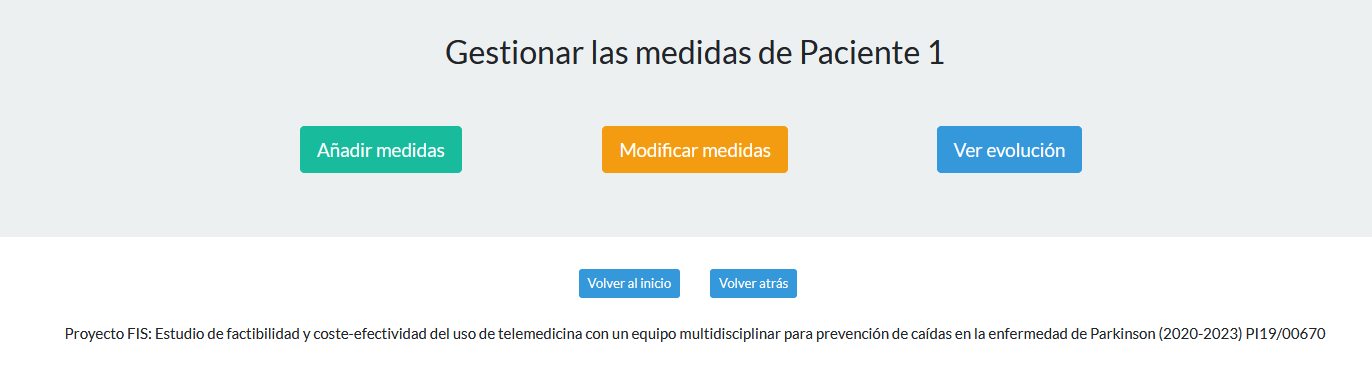
\includegraphics[width=1\textwidth]{menuestad}
	\caption{Menú de estadísticas.}
	\label{fig:menuest}
\end{figure}

\begin{figure}[h]
	\centering
	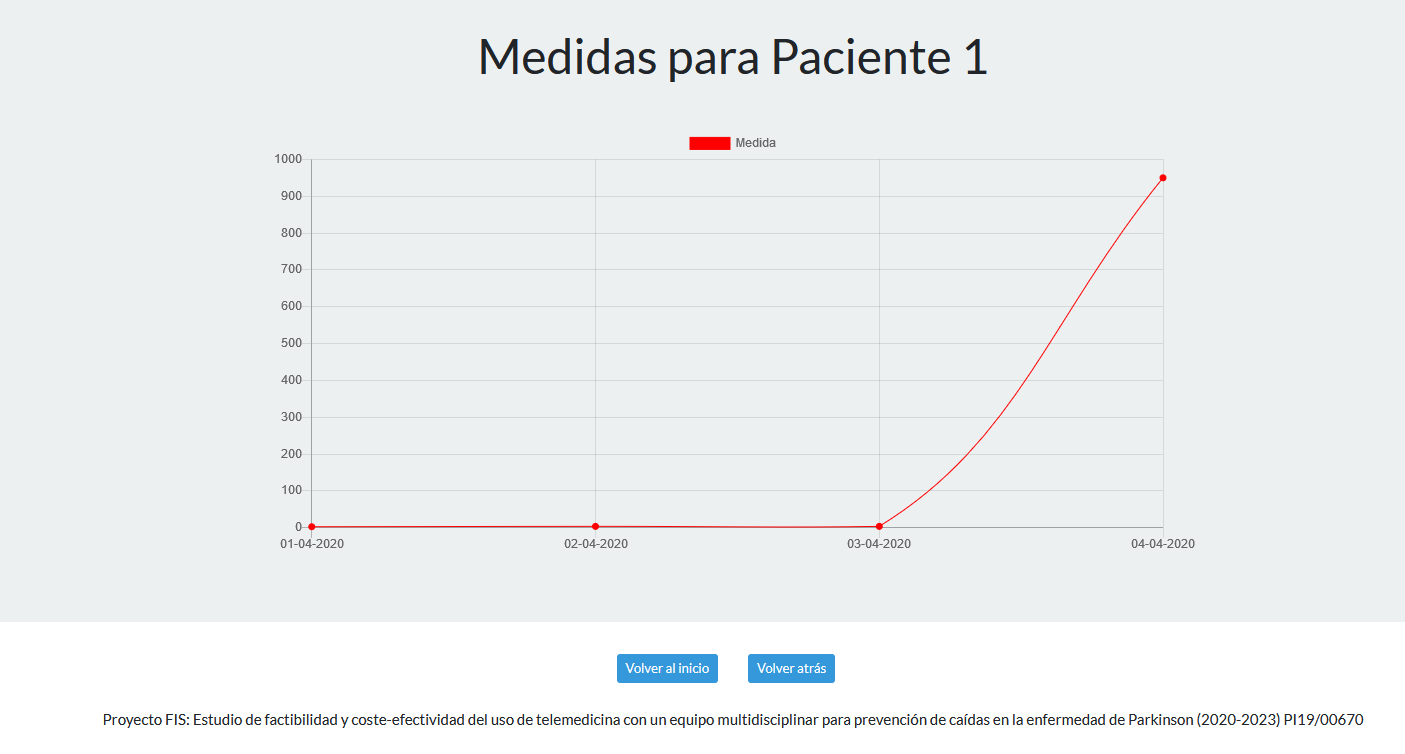
\includegraphics[width=1\textwidth]{ejemploest}
	\caption{Ejemplo de la evolución de un paciente vista por un responsable.}
	\label{fig:ejemploest}
\end{figure}

\subsection{Paciente}
Los pacientes que van a utilizar la aplicación, son pacientes de edad avanzada con Parkinson, y muchos de un estadío avanzado. Es por ello que el diseño de la aplicación se orientó principalmente en la sencillez y facilidad de uso para estos pacientes.

Para poder realizar una aplicación lo más accesible posible primero se ha de saber la forma que van a tener los pacientes de interactuar con ésta. En este caso los pacientes van a utilizar un mando de SNES\footnote{SNES: \textit{Super Nintendo Entertainment System}.} con botones de colores, es por ello que se ha aprovechado estos colores para poder mostrar en la interfaz de la aplicación el botón que han de pulsar para realizar la acción. Además, se ha creado un botón de ayuda que carga una página donde se puede ver la acción que realiza cada botón del mando. Un ejemplo de la interfaz de esta aplicación se puede ver en la figura~\ref{fig:menupaciente}.

\begin{figure}[h]
	\centering
	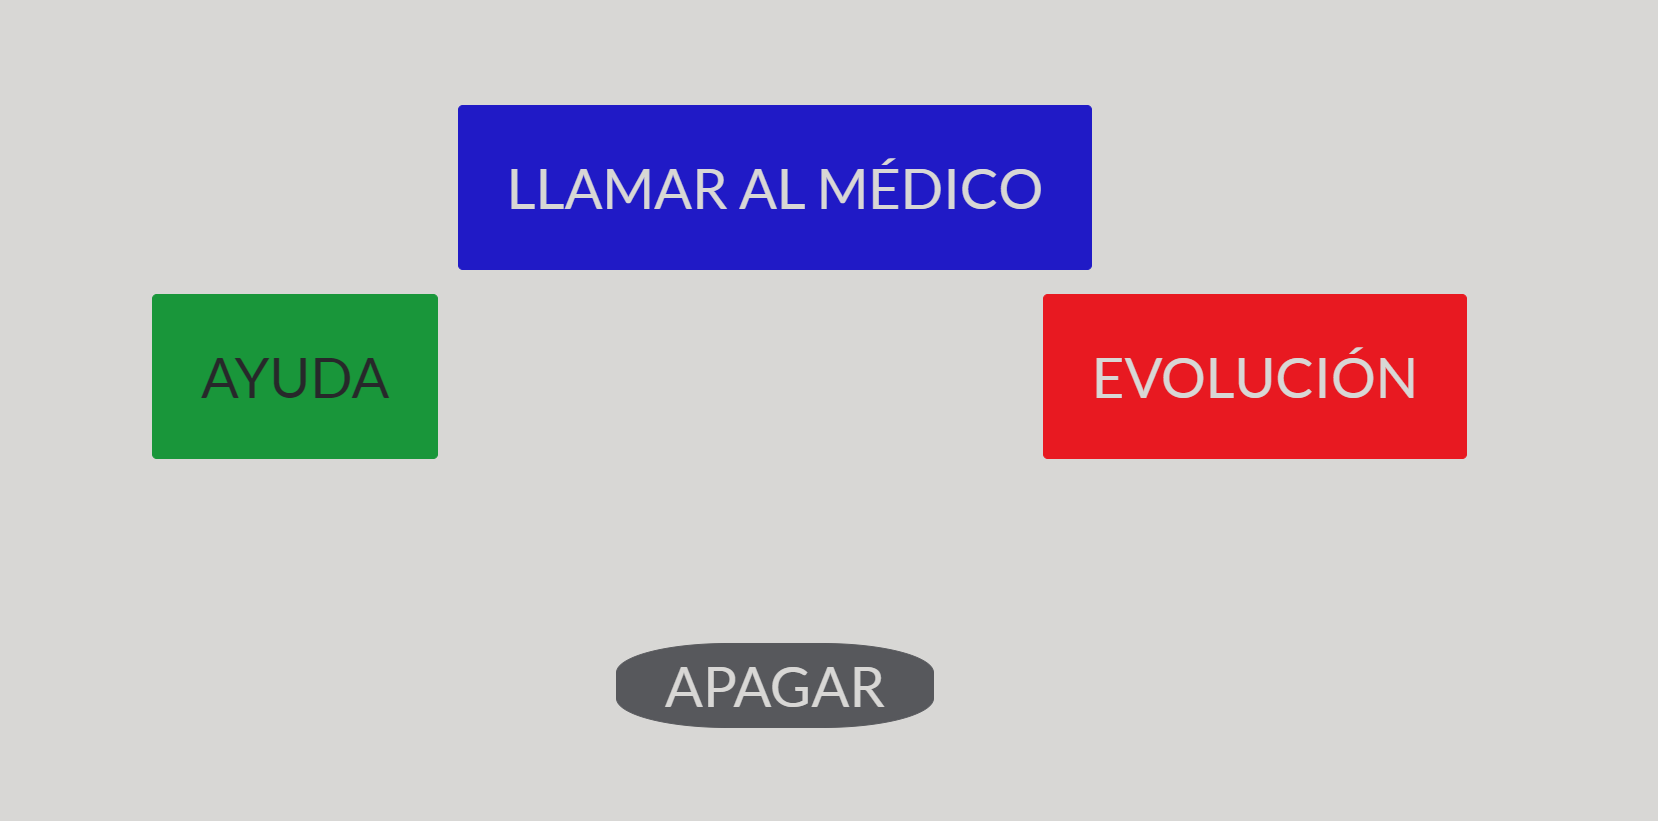
\includegraphics[width=1\textwidth]{menupac}
	\caption{Menú principal de los pacientes.}
	\label{fig:menupaciente}
\end{figure}

\subsection{Dispositivos necesarios}
Para poder utilizar la aplicación se necesitan distintos dispositivos, que dependiendo del tipo de usuario (responsable o paciente) son unos u otros.

Para los responsables lo único que se necesita es un ordenador con conexión a \textit{Internet} y una cámara conectada a éste.

Por otro lado, se presupone que los pacientes no disponen de ningún dispositivo capaz de cargar la aplicación, es por ello que a cada paciente se le proporciona:
\begin{itemize}
	\item Dispositivo: MSI - Cubi N 8GL-001BEU N4000 1,10 GHz Western Digital - Green M.2 120 GB Serial ATA III.
	\item Cámara: Logitech HD Pro WebCam C920.
\end{itemize}

\subsection{Conexión}
Como ya se ha comentado, el principal uso de la aplicación es la realización de rehabilitación \textit{online} para pacientes, mayoritariamente de tercera edad, que no se pueden desplazar a las consultas. Muchas de estas personas mayores viven en lugares donde no se tiene contratada ninguna línea de \textit{Internet}, es por ello que además del desarrollo de la aplicación se contrataron una serie de \textit{routers} 4G para poder proporcionar conexión a los dispositivos necesarios. 

\section{Investigación de algoritmos de visión por computador} \label{aspc}
Tras haber desarrollado la versión inicial, donde en un futuro se quiere añadir los resultados de este proyecto, se pasó a realizar la primera investigación sobre los distintos algoritmos de visión por computador capaces de detectar y seguir los movimientos de una persona. 

De estos algoritmos se necesita:
\begin{itemize}
	\item Posibilidad de cargar un modelo existente o crear un modelo capaz de detectar a la persona que sale en la imagen.
	\item Posibilidad de cargar un modelo existente o crear un modelo capaz de detectar la posición de la persona.
	\item Que el procesado de nuevos fotogramas para detectar a la persona y su posición se realice en poco tiempo.
	\item Que la salida del procesado de los fotogramas pueda servir para una posterior comparación con el ejercicio base.
\end{itemize}

Teniendo todos estos factores en cuenta, se estudió qué herramientas se pueden usar para esta fase del trabajo. Se buscaron herramientas programadas en \textit{Python} para poder integrarse bien con el resto del proyecto y porque es uno de los lenguajes con los cuales se tiene más soltura, tanto por parte del alumno como por parte de los tutores para resolver dudas y ayudar en los problemas. Las herramientas encontradas fueron:
\begin{itemize}
	\item \textit{TF-Pose-Estimator}.
	\item \textit{PoseNet}.
	\item \textit{Detectron2}.
\end{itemize}

De cada una de estas herramientas se realizó una investigación y experimentación para evaluar si cumplían las necesidades requeridas. Al finalizar esta etapa, la única herramienta que cumplía con todas las necesidades era \textit{Detectron2}. Además, permite con un modelo ya creado por los propios desarrolladores realizar las tareas de predicción de elementos y de la posición de la persona.

Cabe destacar uno de los grandes problemas que surgió en esta fase, y fue justamente con \textit{Detectron2}, la herramienta elegida. El problema era que las versiones de \textit{CUDA} y de \textit{PyTorch} no eran compatibles. El problema se agrandó al estar trabajando en un \textit{workstation} de la universidad como es \textit{Gamma} que utilizan otros investigadores y también por la compleja estructura del propio computador. Tras hablar con el administrador de la computadora, que es uno de los tutores de este trabajo, el doctor Álvar Arnaiz González, se pudo arreglar el problema actualizando la versión de los \textit{drivers} de \textit{CUDA}, y una vez actualizados descargando la versión compatible de \textit{PyTorch}. 
\section{Investigación de \textit{Detectron2}}
La fase de investigación de \textit{Detectron2} fue una de las más importantes, y por ende, más costosas en tiempo. Fue en esta fase donde se investigaron las distintas formas que tiene la herramienta para crear o importar modelos con los que poder trabajar. Una vez se seleccionó el modelo se realizó otro estudio para ver qué configuración era la más correcta en el problema tratado.

Al ser una de las fases en las que más tiempo se ha dedicado, también es una de las fases donde surgieron más problemas tanto en la creación de los modelos, como en la visualización y el almacenamiento de los resultados obtenidos. Todos estos problemas serán comentados en este apartado.  
\subsection{Selección del modelo}
Tras haber elegido a \textit{Detrectron2} como herramienta de visión por computador para detectar a los pacientes y obtener de estos sus posiciones, había que elegir qué modelo, dentro de las posibilidades de la herramienta, utilizar para realizar estas tareas.

\textit{Dectectron2} permite dos formas de obtener un modelo:
\begin{itemize}
	\item Crear un modelo propio a partir de una gran cantidad de datos.
	\item Importación de modelos ya entrenados.
\end{itemize}

Ante la falta de datos para la creación de un modelo que diese buenos resultados, y al comprobar en la fase anterior que con la importación de modelos existentes se podían obtener buenos resultados, la investigación se centró en los modelos ya existentes entrenados por los creadores de la herramienta. Estos modelos de redes neuronales fueron entrenados en servidores \textit{Big Basin} de \textit{Facebook}, sucesores de los servidores \textit{Big Sur}, ambos orientados al uso de arquitecturas con varias GPUs potentes para el entrenamiento y uso de algoritmos de inteligencia artificial~\cite{bigbasin}. En concreto, estos modelos fueron entrenados con 8 Nvidia Tesla V100 con \textit{NVLink}, una tecnología que mejora las interconexiones entre GPUs proporcionando mayor ancho de banda, haciendo el sistema más escalable~\cite{nvlink}. La mejora con otras generaciones de comunicación \textit{inter-GPU} se puede ver en la figura~\ref{fig:nvlink}.

\begin{figure}[h]
	\centering
	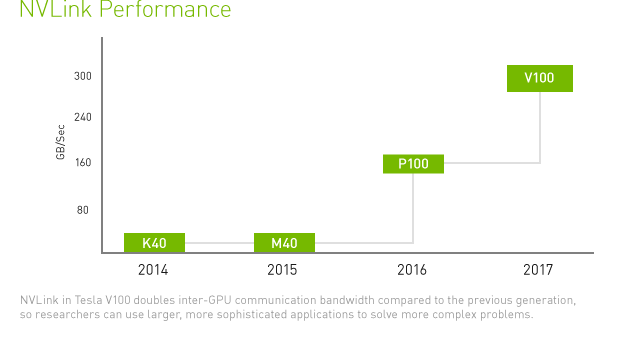
\includegraphics[width=1\textwidth]{nvlink}
	\caption[Mejora del rendimiento en GB/s con NVlink.]{Mejora del rendimiento en GB/s con NVlink~\cite{nvlink}.}
	\label{fig:nvlink}
\end{figure}

Los modelos creados en \textit{Detectron2} se diferencian en los siguientes tipos:
\begin{itemize}
	\item COCO Detection with Faster R-CNN (Figura~\ref{fig:faster_rcnn_R_50_C4_1x}): modelo que predice los objetos y personas de la imagen.

	\item COCO Detection with RetinaNet (Figura~\ref{fig:retinanet_R_101_FPN_3x}): modelo que detecta objetos y personas. Como se puede ver en la imagen de ejemplo, la interpretación no es buena aun utilizando un \textit{threshold} alto.

	\begin{figure}[ht]
		\begin{subfigure}{.48\textwidth}
			\centering
			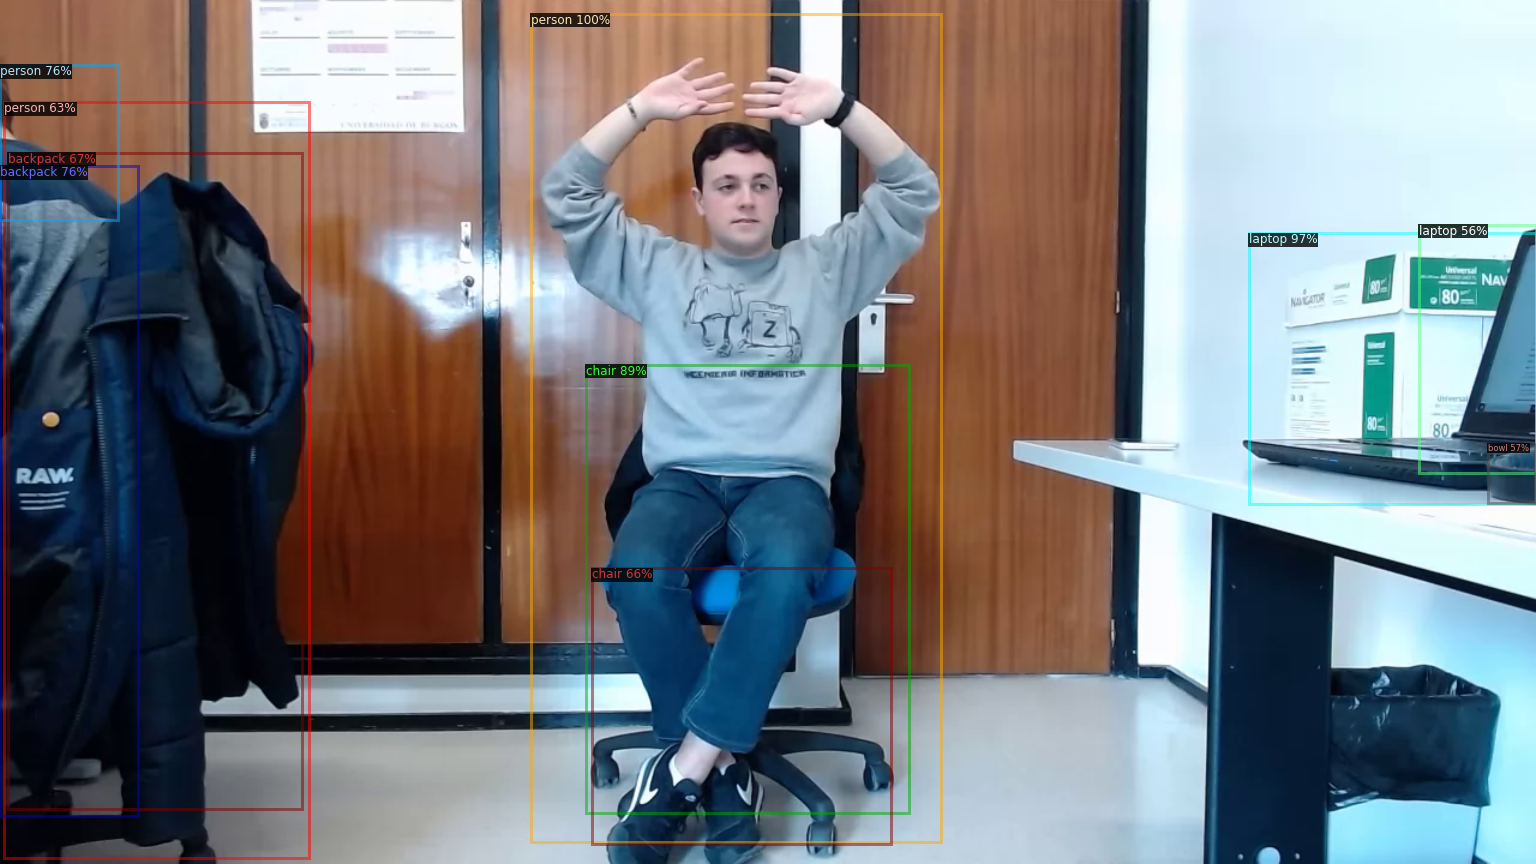
\includegraphics[width=1\textwidth]{faster_rcnn_R_50_C4_1x}
			\caption{Modelo COCO Detection Faster R-CNN, \texttt{faster\_rcnn\_R\_50\_C4\_1x}.}
			\label{fig:faster_rcnn_R_50_C4_1x}
		\end{subfigure}
		\begin{subfigure}{.48\textwidth}
			\centering
			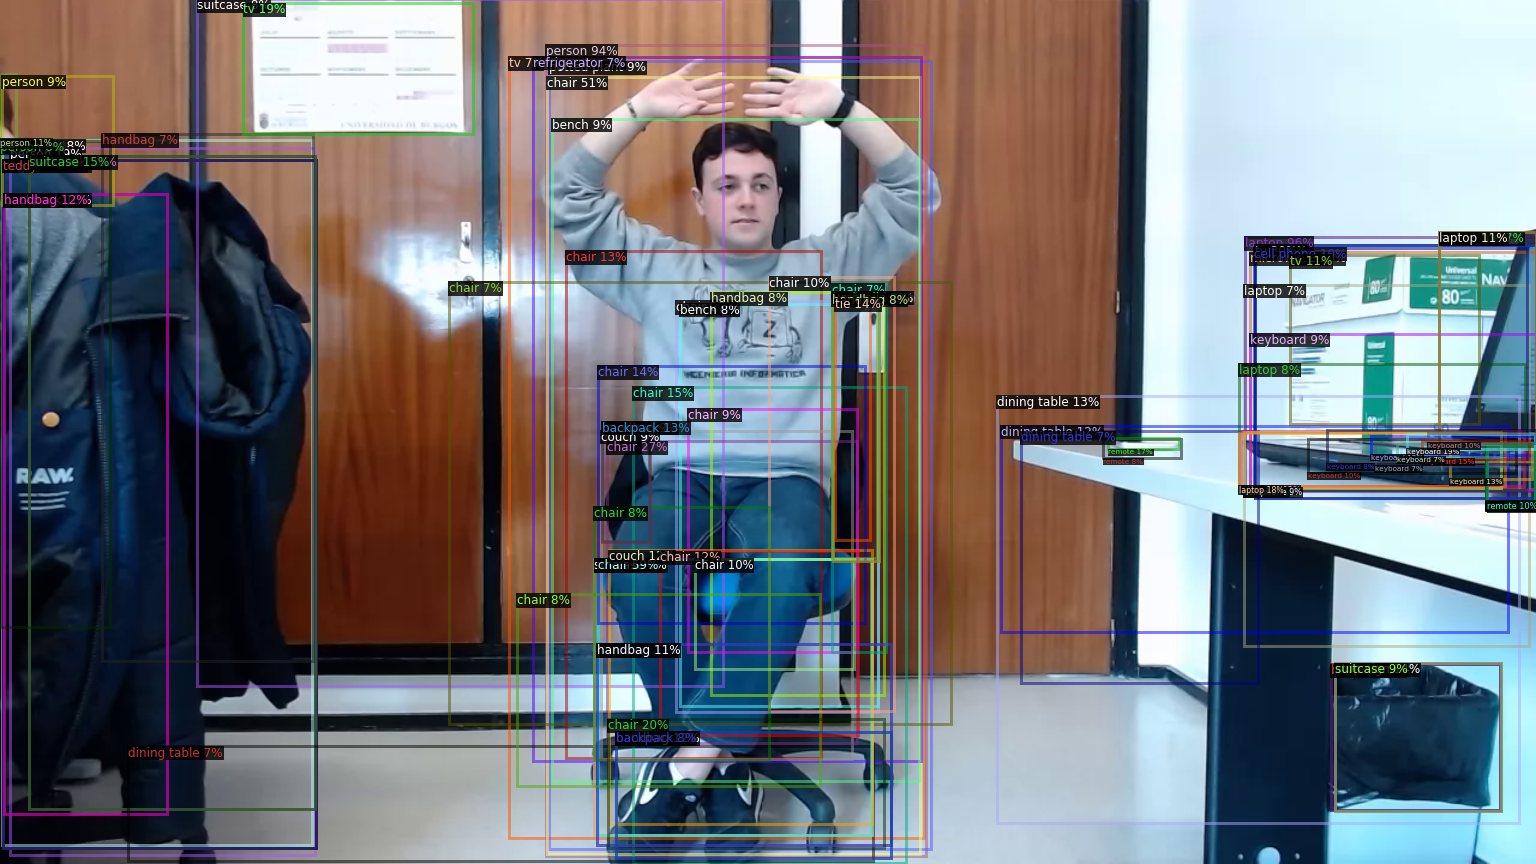
\includegraphics[width=1\textwidth]{retinanet_R_101_FPN_3x}
			\caption{Modelo COCO Detection with RetinaNet, \texttt{retinanet\_R\_101\_FPN\_3x}.}
			\label{fig:retinanet_R_101_FPN_3x}
		\end{subfigure}
		\caption{Modelos \textit{Detectron2}.}
		\label{fig:m1}
	\end{figure}
	\item COCO Detection with RPN and Fast R-CNN: modelos que no se han conseguido probar ya que no siguen la misma estructura que el resto de modelos.
	\item COCO Instance Segmentation Baselines with Mask R-CNN (Figura~\ref{fig:mask_rcnn_R_50_DC5_3x}): modelos de detección de objetos y persona, con delimitación en el área ocupada.

	\item COCO Person Keypoint Detection Baselines with Keypoint R-CNN (Figura~\ref{fig:keypoint_rcnn_R_101_FPN_3x}): modelos que detectan a las posiciones y unos puntos claves de ellas, estos puntos son nariz, ojos, orejas, hombros, codos, muñecas, cadera, rodilla y tobillos. Como se puede ver en la imagen de ejemplo, estos modelos predicen bastante bien la posición, pero a veces detectan otras cosas como personas, por lo que se posteriormente se vio necesario un estudio sobre el \textit{threshold}.

	\begin{figure}[ht]
		\begin{subfigure}{.48\textwidth}
			\centering
			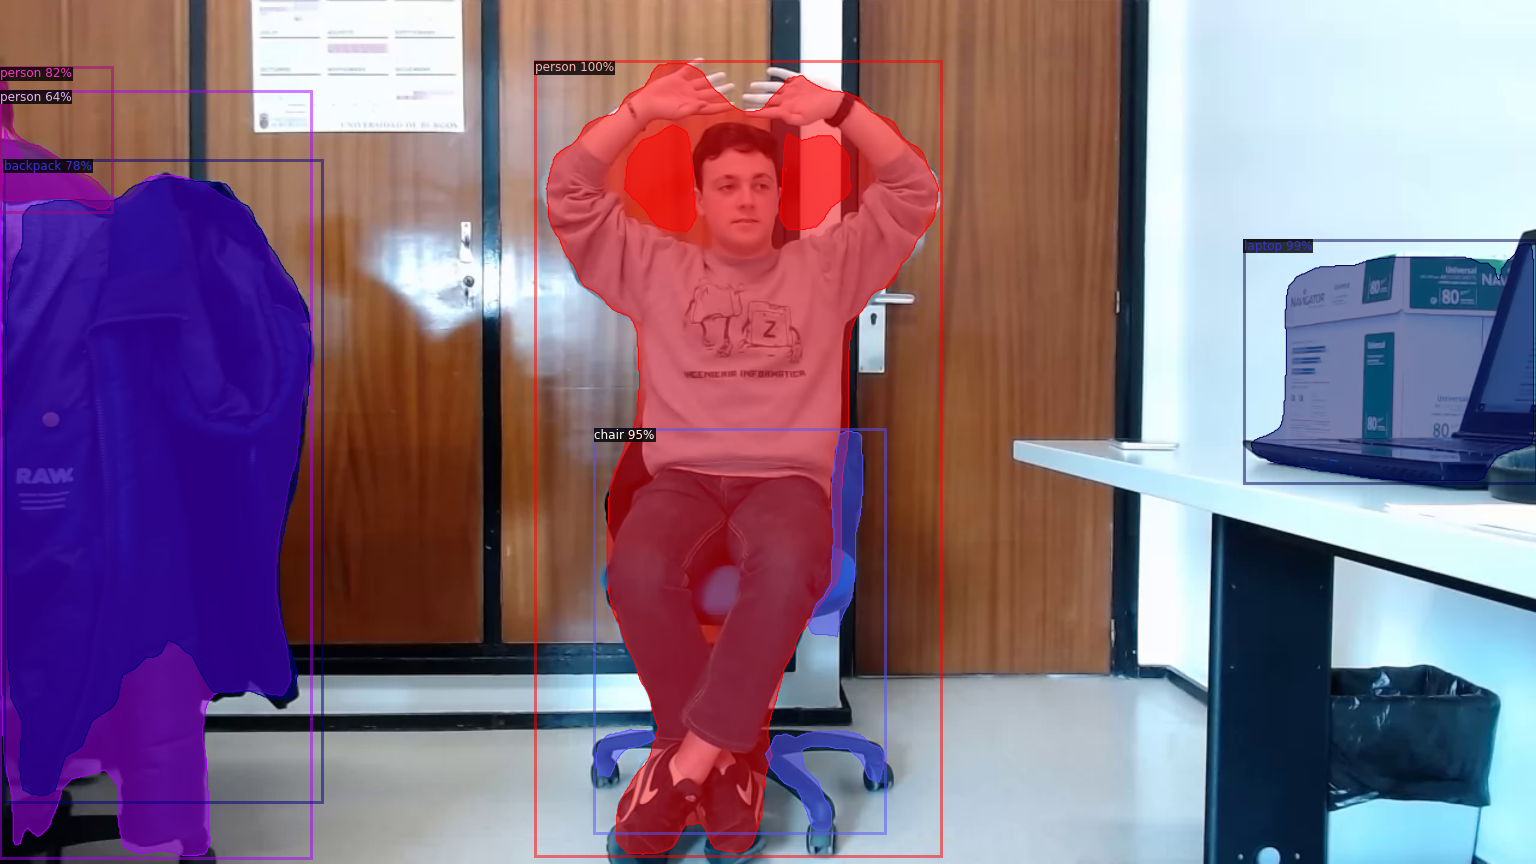
\includegraphics[width=1\textwidth]{mask_rcnn_R_50_DC5_3x}
			\caption{Modelo COCO Instance Segmentation Baselines with Mask R-CNN, \texttt{mask\_rcnn\_R\_50\_DC5\_3x}.}
			\label{fig:mask_rcnn_R_50_DC5_3x}
		\end{subfigure}
		\begin{subfigure}{.48\textwidth}
			\centering
			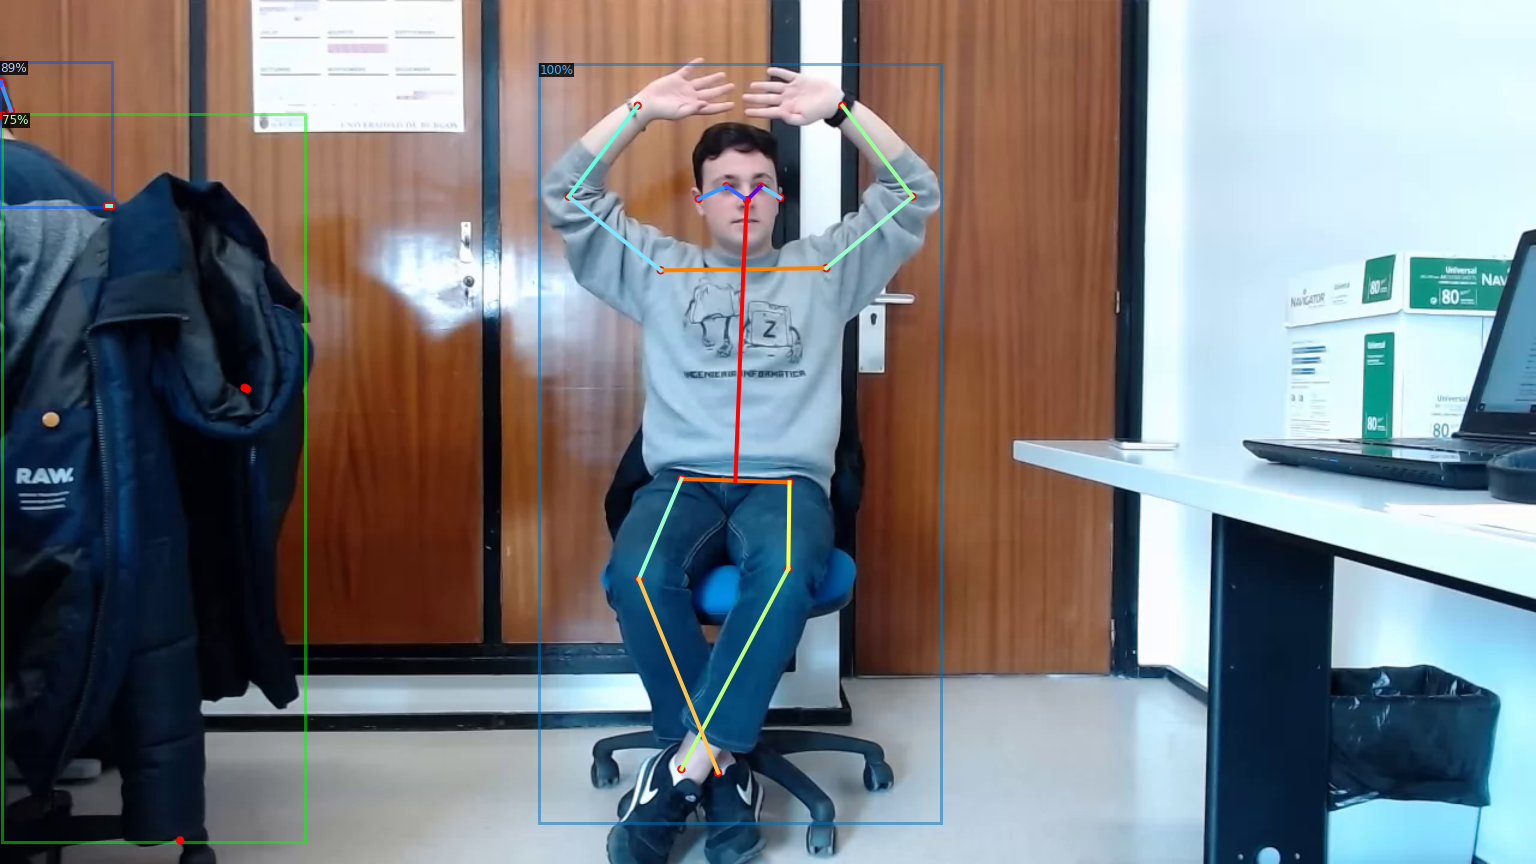
\includegraphics[width=1\textwidth]{keypoint_rcnn_R_101_FPN_3x}
			\caption{Modelo COCO Person Keypoint Detection Baselines with Keypoint R-CNN, \texttt{keypoint\_rcnn\_R\_101\_FPN\_3x}.}
			\label{fig:keypoint_rcnn_R_101_FPN_3x}
		\end{subfigure}
		\caption{Modelos \textit{Detectron2}.}
		\label{fig:m2}
	\end{figure}
	\item COCO Panoptic Segmentation Baselines with Panoptic FPN (Figura~\ref{fig:panoptic_fpn_R_101_3x}): modelos de segmentación como COCO Instance Segmentation Baselines with Mask R-CNN, obtienen resultados muy parecidos.

	\item LVIS Instance Segmentation Baselines with Mask R-CNN (Figura~\ref{fig:mask_rcnn_X_101_32x8d_FPN_1x}): modelos orientados a la detección de objetos, necesitan un \textit{threshold} bajo para detectar diversos objetos.

	\begin{figure}[ht]
		\begin{subfigure}{.48\textwidth}
			\centering
			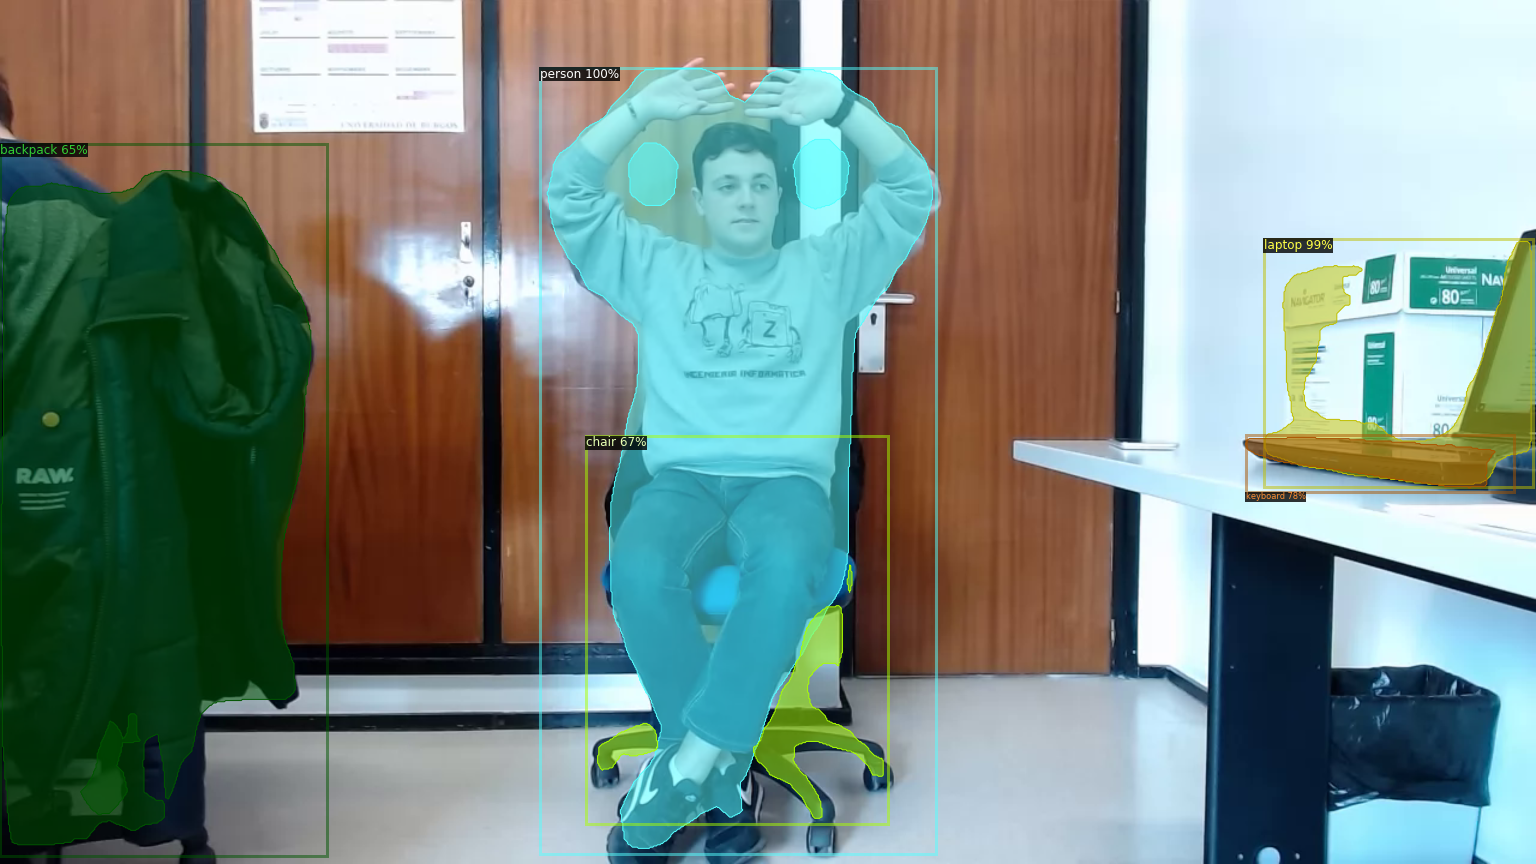
\includegraphics[width=1\textwidth]{panoptic_fpn_R_101_3x}
			\caption{Modelo COCO Panoptic Segmentation Baselines with Panoptic FPN, \texttt{panoptic\_fpn\_R\_101\_3x}.}
			\label{fig:panoptic_fpn_R_101_3x}
		\end{subfigure}
		\begin{subfigure}{.48\textwidth}
			\centering
			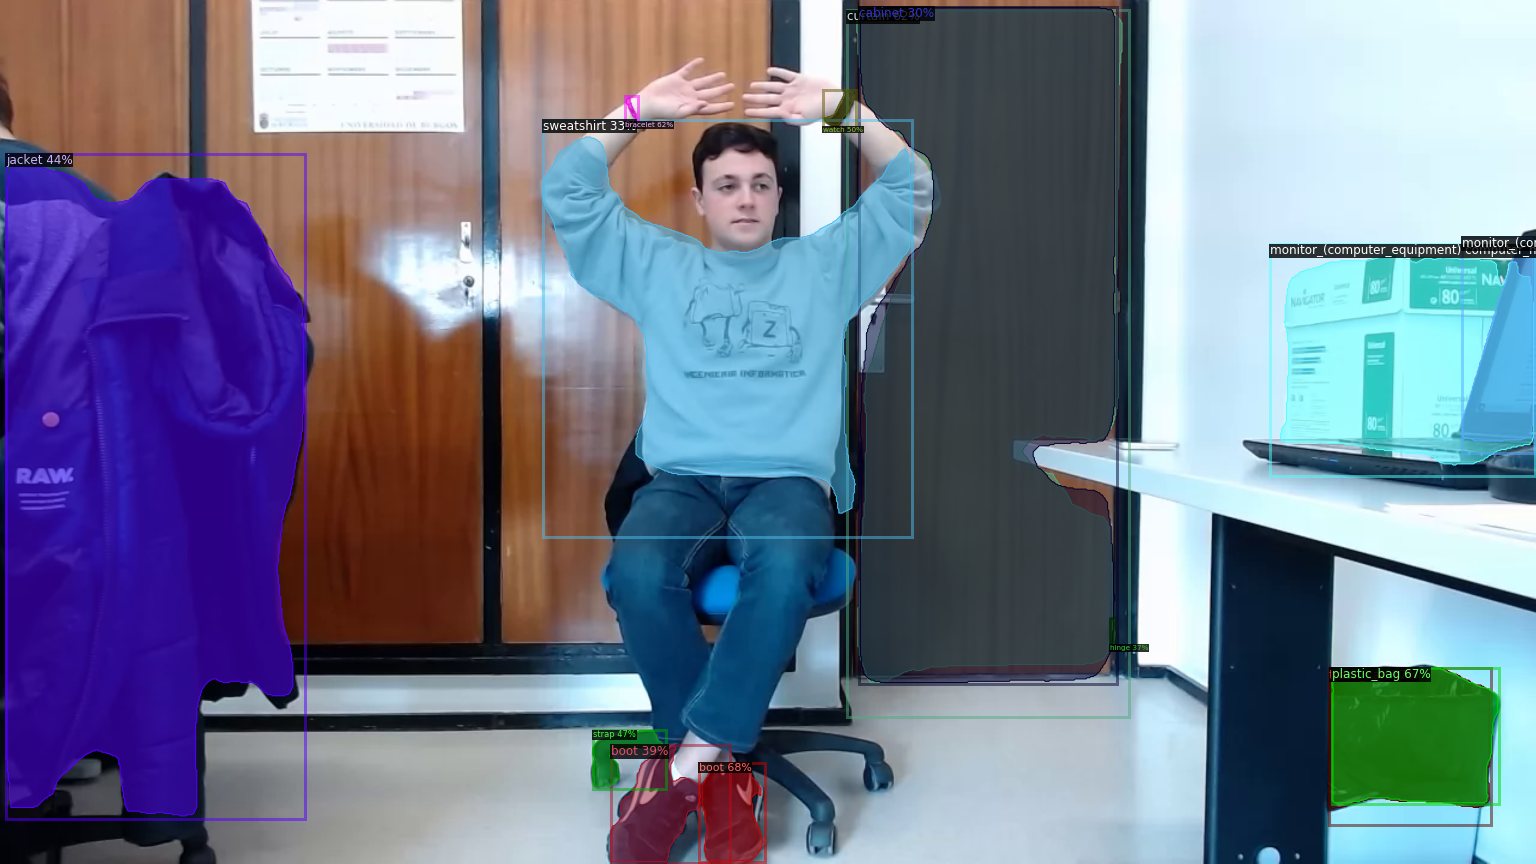
\includegraphics[width=1\textwidth]{mask_rcnn_X_101_32x8d_FPN_1x}
			\caption{Modelo LVIS Instance Segmentation Baselines with Mask R-CNN, \texttt{mask\_rcnn\_X\_101\_32x8d\_FPN\_1x}.}
			\label{fig:mask_rcnn_X_101_32x8d_FPN_1x}
		\end{subfigure}
		\caption{Modelos \textit{Detectron2}.}
		\label{fig:m3}
	\end{figure}
	\item Por último se encuentran modelos como Cityscapes \& Pascal VOC Baselines, otras configuraciones y algoritmos de la primera versión de la herramienta \textit{Detectron}. Estos modelos son muy parecidos a los ya mostrados.
\end{itemize}

Con el estudio de todos los modelos existentes en \textit{Detectron2}, se ha comprobado como los únicos modelos que sirven para el problema planteado son COCO Person Keypoint Detection Baselines with Keypoint R-CNN. Dentro de este tipo de modelos existen un total de 4 modelos distintos. Para la elección del mejor de estos modelos se realizó otro estudio, esta vez comprobando los tiempos de ejecución, ya que todos los modelos de este tipo realizan unas buenas predicciones (principalmente porque el problema es sencillo, al tener a la persona en el centro de la imagen).

Para realizar este estudio se analizó el tiempo de procesado e impresión de varios vídeos con cada uno de los modelos. Para ello se calcularon estos valores para los 4 posibles modelos con un total de 7 vídeos. De este estudio se obtuvieron los resultados que se pueden ver en la tabla~\ref{tab:modelos}.

\begin{table}[h]
	\centering
	\resizebox{\columnwidth}{!}{
\begin{tabular}{l | rrrr}
	\toprule
	\textbf{Modelo} &     \textbf{T. Carga (ms)} &       \textbf{T. Procesamiento (ms)} &  \textbf{N. Fotogramas} &     \textbf{Periodo} \\
	\midrule
	\texttt{keypoint\_rcnn\_R\_50\_FPN\_1x}      &   $8083.19$ &  $216519.97$ &     $1989$ &  $108.86$ \\
	\texttt{keypoint\_rcnn\_R\_50\_FPN\_3x}     &   $7539.65$ &  $216625.36$ &     $1989$ &  $108.91$ \\
	\texttt{keypoint\_rcnn\_R\_101\_FPN\_3x}     &  $9806.49$ &  $259716.33$ &     $1989$ &  $130.58$ \\
	\texttt{keypoint\_rcnn\_X\_101\_32x8d\_FPN\_3x} &  $14853.03$ &  $407086.70$	 &     $1989$ &  $204.67$ \\
	\bottomrule
\end{tabular}
}
\caption{Tabla con el estudio de los modelos de posición ordenado por periodo.}
\label{tab:modelos}
\end{table}

Como se puede observar, los datos obtenidos para los modelos son muy parecidos, sobre todo para los dos con menor periodo ($T. Proc./Fotogramas$). Tras observar los datos se decidió elegir el modelo \texttt{keypoint\_rcnn\_R\_50\_FPN\_3x} (es además el modelo con el que se hicieron las primera pruebas y con el que se decidió a \textit{Detectron2} como herramienta para detectar el movimiento) para utilizarlo en el resto del proyecto. Se eligió este modelo debido a que, aunque es el segundo con el periodo más bajo con una diferencia casi inapreciable de $0.05$ milisegundos, su tiempo de carga es de medio segundo inferior al modelo con el mejor tiempo de procesamiento por fotograma.

Además, en este estudio se ha podido comprobar que los modelos trabajan correctamente con independencia del tipo de ropa que lleve la persona o si pasa un objeto por medio de la imagen (normalmente la posición es correcta, pero como se comentará más adelante a veces algunos fotogramas no son correctos), como se pueden ver en la figuras~\ref{fig:chaqueta} y~\ref{fig:caja}.

Se puede comentar que el modelo seleccionado usa una red neuronal piramidal de tipo FPN con ResNet y RCNN para la detección de la persona, y dentro de la persona sus puntos más importantes.

\begin{figure}[ht]
	\begin{subfigure}{.48\textwidth}
		\centering
		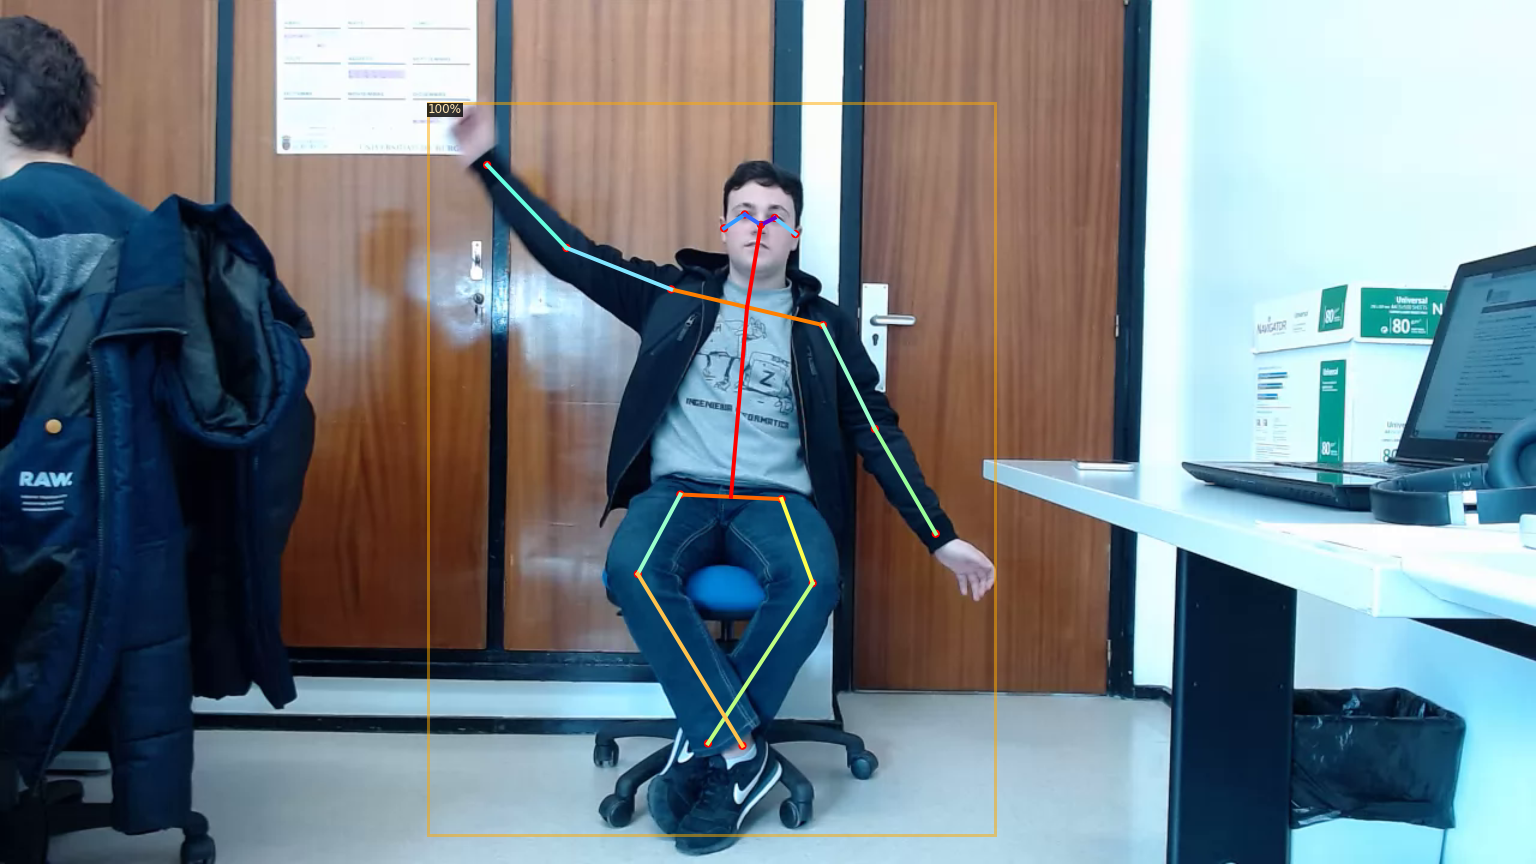
\includegraphics[width=1\textwidth]{chaqueta}
		\caption{Prueba con chaqueta.}
		\label{fig:chaqueta}
	\end{subfigure}
	\begin{subfigure}{.48\textwidth}
		\centering
		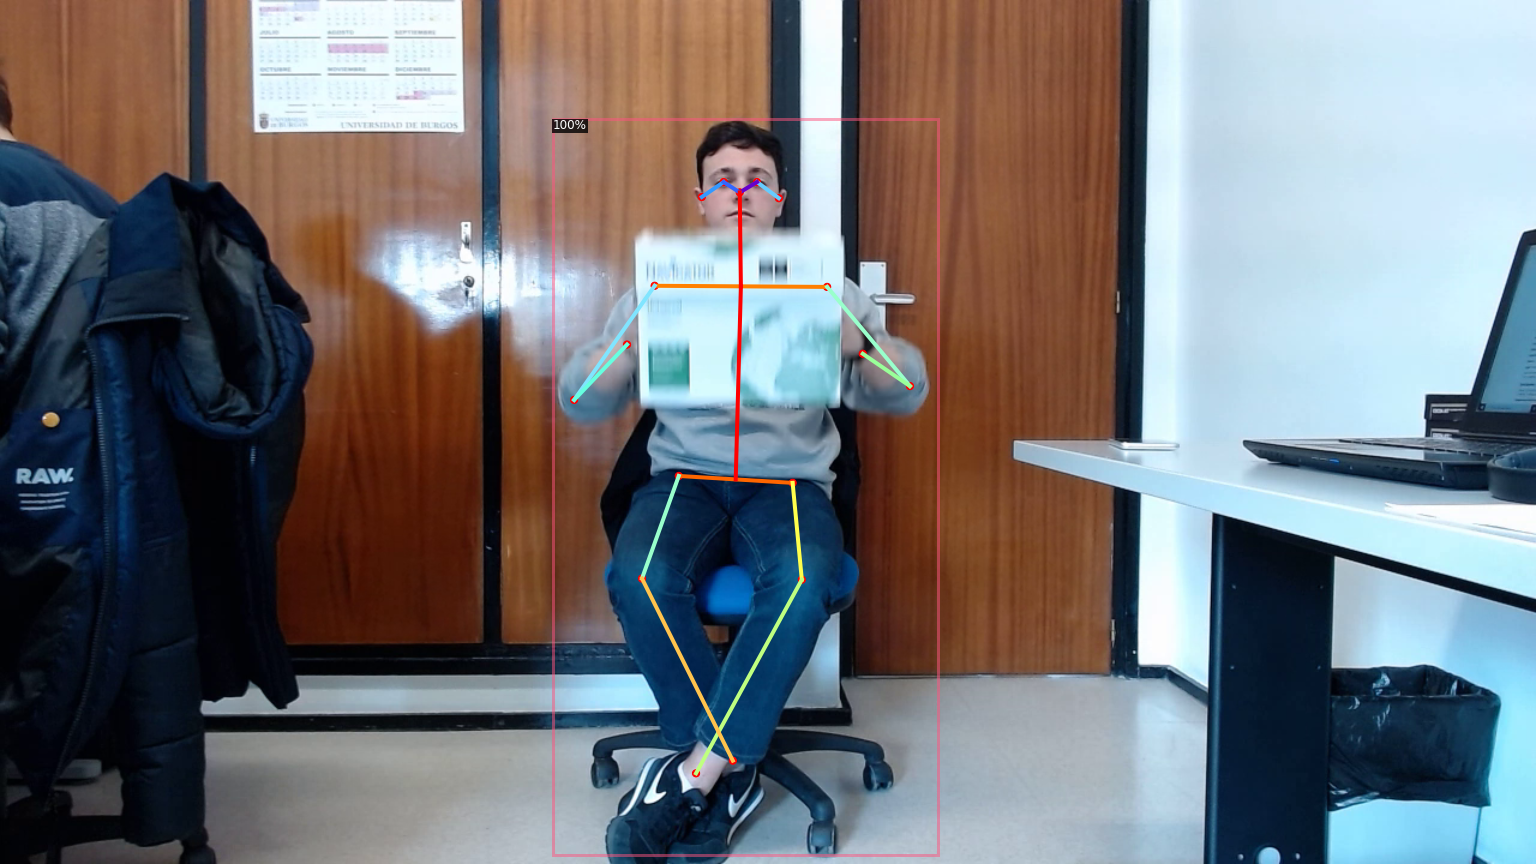
\includegraphics[width=1\textwidth]{caja}
		\caption{Prueba con un objeto de por medio.}
		\label{fig:caja}
	\end{subfigure}
	\caption{Pruebas con ropa y objetos.}
	\label{fig:ropobj}
\end{figure}



\subsection{Definición del \textit{threshold}}
Como se ha comentado en el apartado anterior, es necesario definir un \textit{threshold}, que es un valor entre 0 y 1 que define la sensibilidad del modelo al detectar, es decir, con valores cercanos a 0 el modelo tiende a detectar más elementos (muchos de ellos erróneos) y cuanto más cercano a 1 menos sensible es, solo detectando los elementos más claros. Sobre este valor se ha realizado un estudio de posibles valores, los valores probados fueron $0.3$; $0.5$; $0.75$; $0.99$.

Con valores bajos del \textit{threshold} se observa que se detectan cosas que no son personas, o se detectan personas que no salen completas en la imagen, como se puede observar en el figura~\ref{fig:pruebaCon0.3}. Esto ocurre con los valores $0.3$; $0.5$; $0.75$ que dan la misma salida. Sin embargo, con el valor $0.99$, como se puede ver en la figura~\ref{fig:pruebaCon0.99}, se obtienen muy buenos resultados detectando únicamente a la persona que aparece en el centro de la imagen, con la posición exacta en todos los puntos.

\begin{figure}[ht]
	\begin{subfigure}{.48\textwidth}
		\centering
		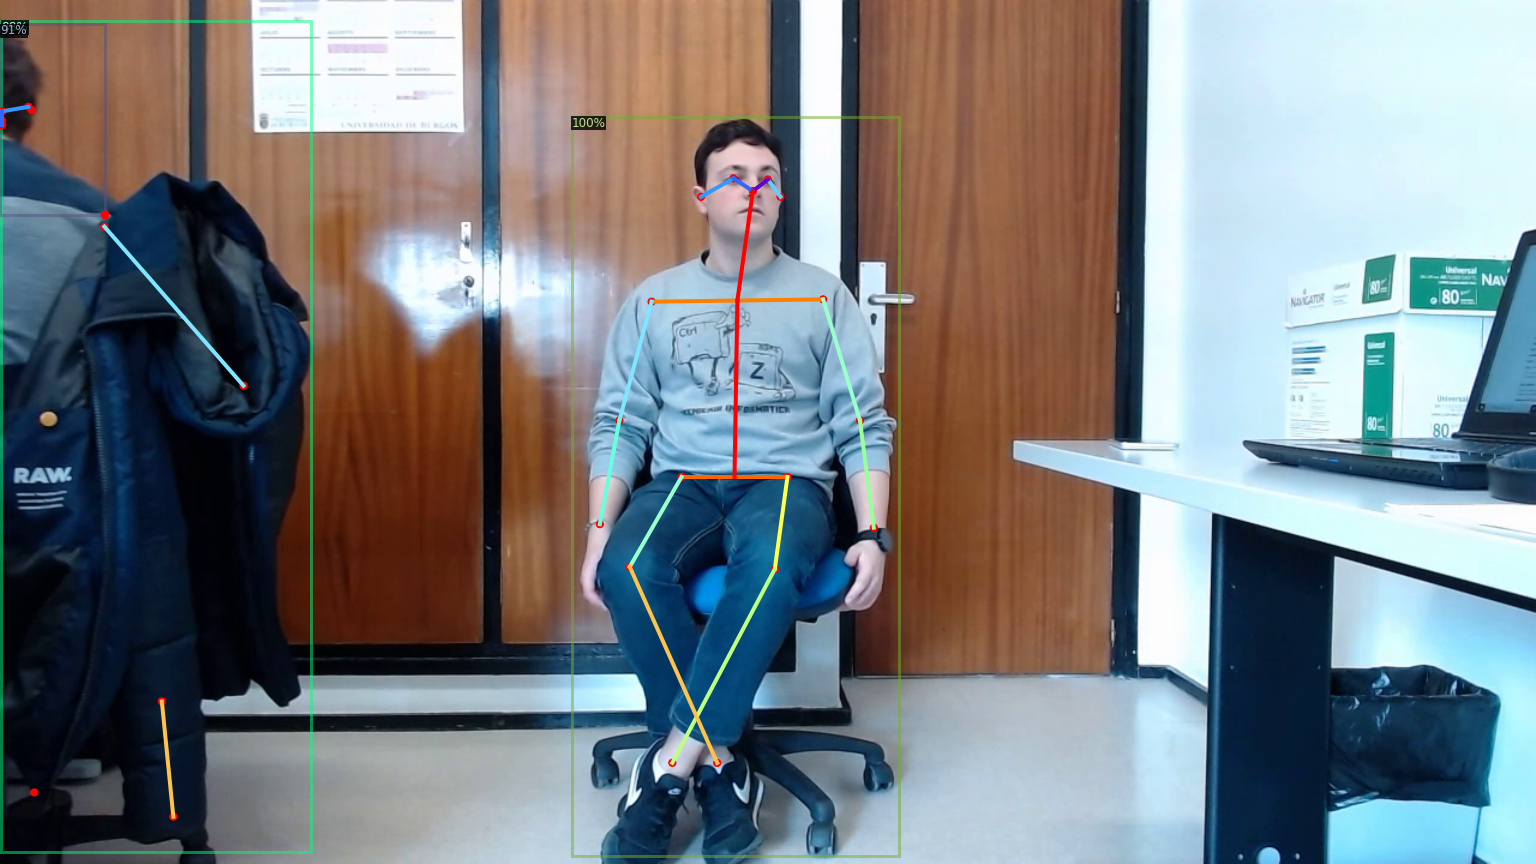
\includegraphics[width=1\textwidth]{pruebaCon0.3}
		\caption{Prueba con \textit{threshold} a $0.3$.}
		\label{fig:pruebaCon0.3}
	\end{subfigure}
	\begin{subfigure}{.48\textwidth}
		\centering
		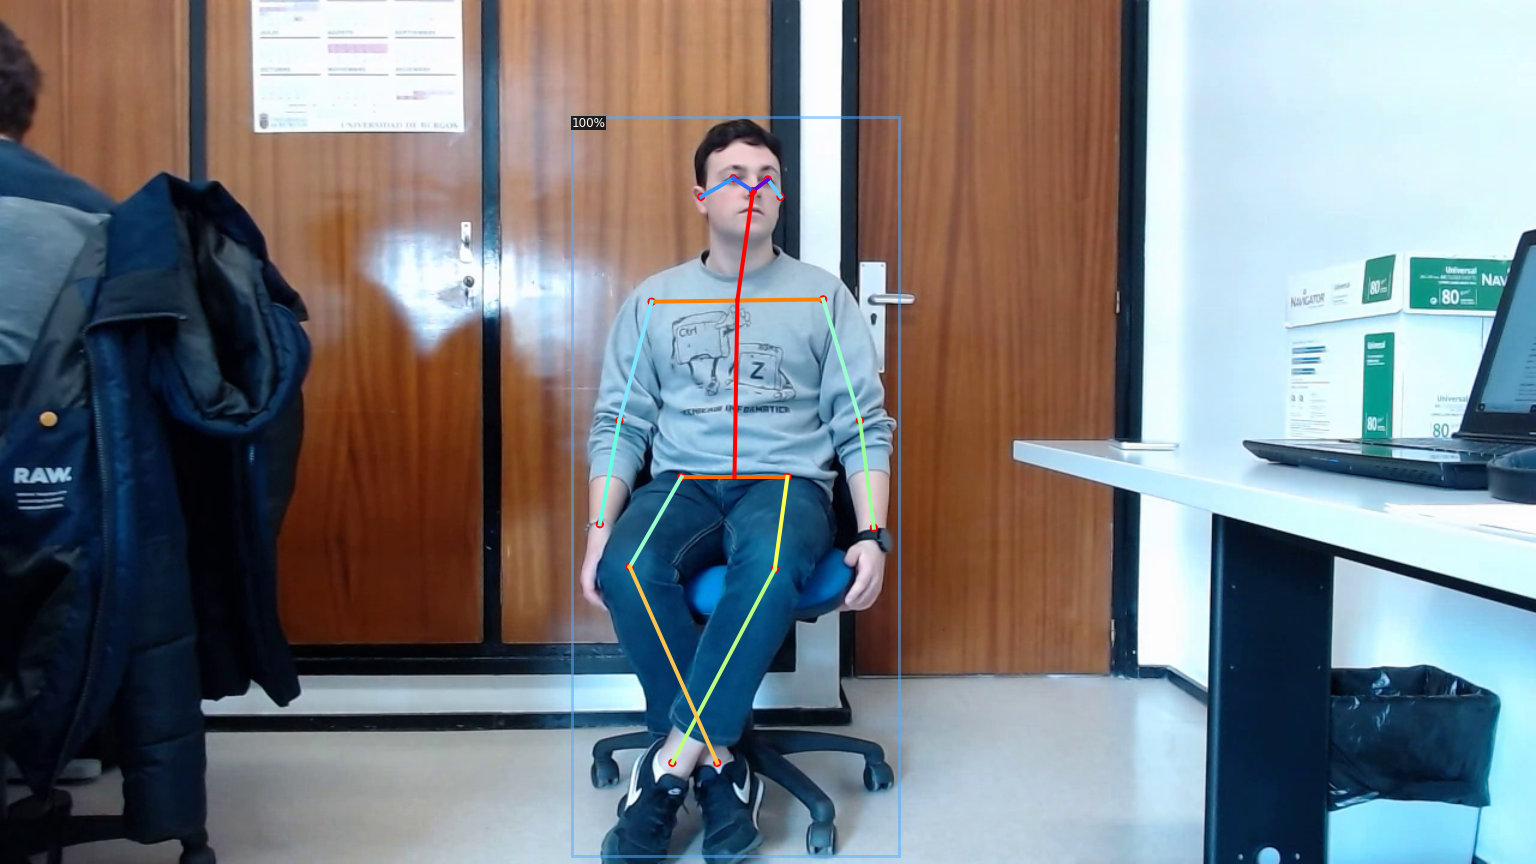
\includegraphics[width=1\textwidth]{pruebaCon0.99}
		\caption{Prueba con \textit{threshold} a $0.99$.}
		\label{fig:pruebaCon0.99}
	\end{subfigure}
	\caption{Pruebas con el \textit{threshold}.}
	\label{fig:thr}
\end{figure}

\subsection{Problemas surgidos}
Como se ha comentado a lo largo del apartado, han surgido distintos problemas que se pueden resumir en:
\begin{itemize}
	\item Problema con los modelos COCO Detection with RPN and Fast R-CNN, que al no tener la misma estructura que el resto de modelos de \textit{Detectron2} no se han podido probar.
	\item Se intentó almacenar los vídeos procesados pero, por problemas con \textit{OpenCV}, no se pudo guardar en esta etapa.
\end{itemize}

\section{Cálculo de características}
Una vez se seleccionó el modelo que se iba a utilizar durante todo el proyecto y se determinó el parámetro \textit{threshold} de los modelos, el siguiente paso fue la interpretación de las salidas del modelo. Y después de haber interpretado con el modelo de \textit{Detectron2} una posición ser capaces de calcular características que definan de la mejor manera los datos.
\subsection{Interpretación de las predicciones}
Si se analiza la salida tras predecir un imagen con el predictor creado (DefaultPredictor), se observa que devuelve un diccionario con una única entrada llamada <<instances>> donde se almacena toda la información. Dentro de la instancia existen los siguientes apartados:
\begin{itemize}
	\item \texttt{pred\_boxes}: Boxes, estructura propia de \textit{Dectectron2} donde se almacenan límites de donde entiende que está la persona en un \textit{tensor}, si se ha detectado más de una persona este Boxes estará formado por varios \textit{tensors}.
	\item \texttt{scores}: \textit{tensor} con las probabilidades de que los elementos sean personas. Es este el valor que se compara con el \textit{threshold} para ver si se considera o no como una persona. Si existe más de un valor estos están ordenados de mayor a menor, este es el orden que se sigue en el resto de valores.
	\item \texttt{pred\_classes}: \textit{tensor} con el índice de la clase, en este caso todos los elementos son 0 ya que solo detecta personas, que se identifican con este índice.
	\item \texttt{pred\_keypoints}: \textit{tensor} con todos los puntos clave de cada elemento (persona) detectada. De cada elemento detectado, si la predicción ha sido correcta, se obtienen un total de 17 puntos, con sus valores $x$ e $y$. Después de investigar el posicionamiento de estos puntos se puede decir, como se ve en la figura~\ref{fig:puntos}, que los puntos representan (teniendo en cuenta que se han detectado todos los puntos y que la persona está mirando de frente al objetivo) las partes que se pueden observar en la tabla~\ref{tab:partes}.
\end{itemize}

\begin{table}[h]
	\centering
	\begin{tabular}{ll}
		\toprule
		\textbf{Id} & \textbf{Parte}\\
		\midrule
		0&Nariz\\
		1 y 2&Ojos (izq. y der.)\\
		3 y 4&Orejas (izq.y der.)\\
		5 y 6&Hombros (izq.y der.)\\
		7 y 8&Codos (izq.y der.)\\
		9 y 10&Muñecas-manos (izq.y der.)\\
		11 y 12&Cadera (izq.y der.)\\
		13 y 14&Rodillas (izq.y der.)\\
		15 y 16&Tobillos (izq.y der.)\\
	\bottomrule
	\end{tabular}
\caption{Tabla con las partes de la posición y su identificador.}
\label{tab:partes}
\end{table}


\begin{figure}[h]
	\centering
	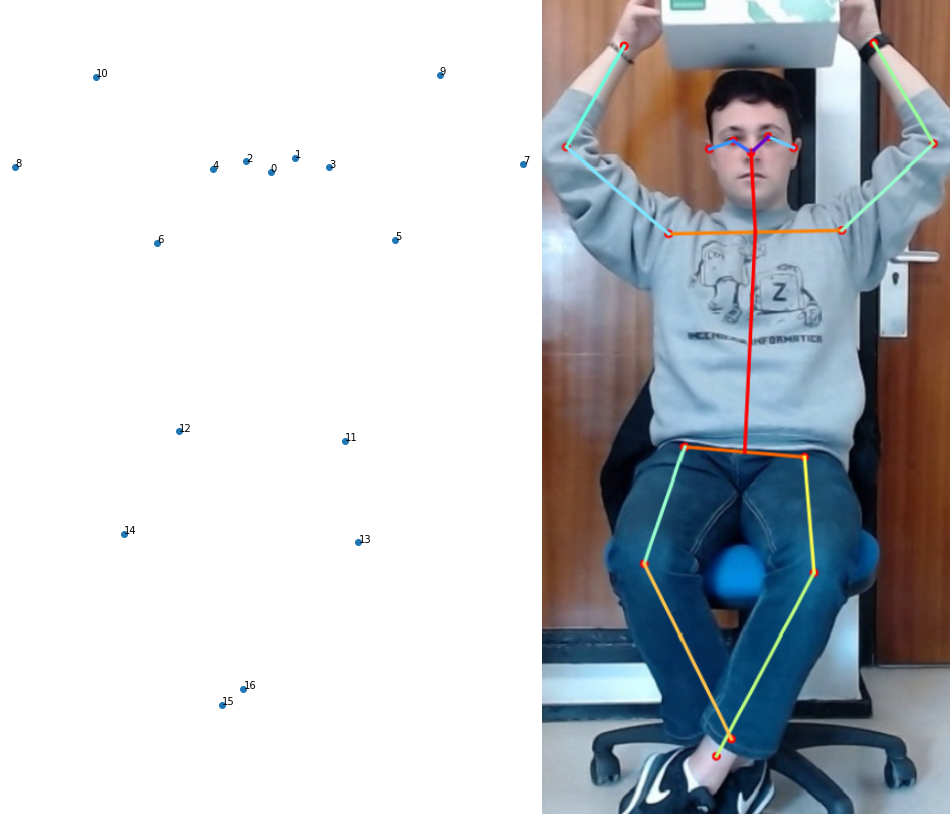
\includegraphics[width=0.75\textwidth]{puntos}
	\caption{Puntos clave predichos con el modelo junto con la etiqueta con su orden.}
	\label{fig:puntos}
\end{figure}
\subsection{Clase de posición}
Una vez se conocen las salidas de las predicciones, se pueden usar estas para obtener más información de la posición de la persona, que en futuras etapas fue usada para la comparación de posiciones. Por ello se creó una clase que almacena todos los puntos detectados además de realizar cálculos para extraer más características.

Para poder obtener más información sobre los puntos se crearon una serie de funciones que permiten:
\begin{itemize}
	\item Cálculo de puntos medios. Este cálculo se realiza para obtener el punto inferior del cuello que se calcula como el punto medio de la recta que une los dos hombros y se utiliza también para calcular el punto central de la cadera a partir de su punto izquierdo y derecho.
	\item Cálculo de la distancia entre puntos. Este punto se ha realizado sobre todos los pares de puntos unidos. Se pueden utilizar para intuir profundidades.
	\item Cálculo de los ángulos en grados. Este cálculo se ha realizado en todas las combinaciones posibles (conjunto de 3 puntos consecutivos), ya que se cree que son las características que más información van a aportar debido a que no dependen de ningún otro valor como puede ser la profundidad a la que está el paciente, su altura...
\end{itemize}

Como se comentó en apartados anteriores, una vez se tienen los puntos, se ha de realizar una serie de comprobaciones para saber si las posiciones son válidas:
\begin{itemize}
	\item Si existe más de una persona detectada se selecciona la primera, ya que es la que tiene un mayor \textit{score} y por lo tanto el modelo cree que puede ser con mayor probabilidad una persona.
	\item Si una predicción no dispone de todos los puntos no se tiene en cuenta. En la práctica con las pruebas que se han realizado esto solo sucede cuando se pasa un objeto por ciertos puntos del cuerpo, cuando ocurre esto hay algunos fotogramas, muy pocos, que no detectan todos los puntos.
\end{itemize}

\section{Primeras versiones comparación de posiciones} \label{PrimeraVersion}
Una vez se había comprobado que el sistema de cálculo de posiciones era correcto se pasó a desarrollar la comparación de posiciones. Para esta primera versión de la comparación de posiciones se decidió usar los ángulos calculados a partir de los puntos y puntos medios de las posiciones, ya que es la única medida calculada que no depende de la posición del usuario grabado.
\subsection{División de la comparación}
La principal característica, aparte del uso de los ángulos, de la primera versión de la comparación de posiciones fue la división de la comparación en distintas partes para poder dar un peso mayor o menor a cada una de ellas. Esta división se creyó necesaria tras observar los vídeos de ejemplos de los ejercicios que se proporcionaron, ya que había ejercicios donde se centraban en los brazos, otros en las piernas\ldots

La división que se planteó en esta versión fue (Figura~\ref{fig:estiradosAbajo2}):
\begin{itemize}
	\item Brazos: en esta parte se encuentran únicamente los ángulos de los codos de ambos brazos (5 y 6).
	\item Torso: ángulos de la cadera con la columna (7 y 8), ángulos de los hombros (3 y 4) y ángulos del cuello con respecto a los hombros (1 y~2).
	\item Piernas: ángulos de la cadera con el fémur de cada pierna (9 y 10) y ángulos de cada rodilla (11 y 12).
\end{itemize}

\begin{figure}[h]
	\centering
	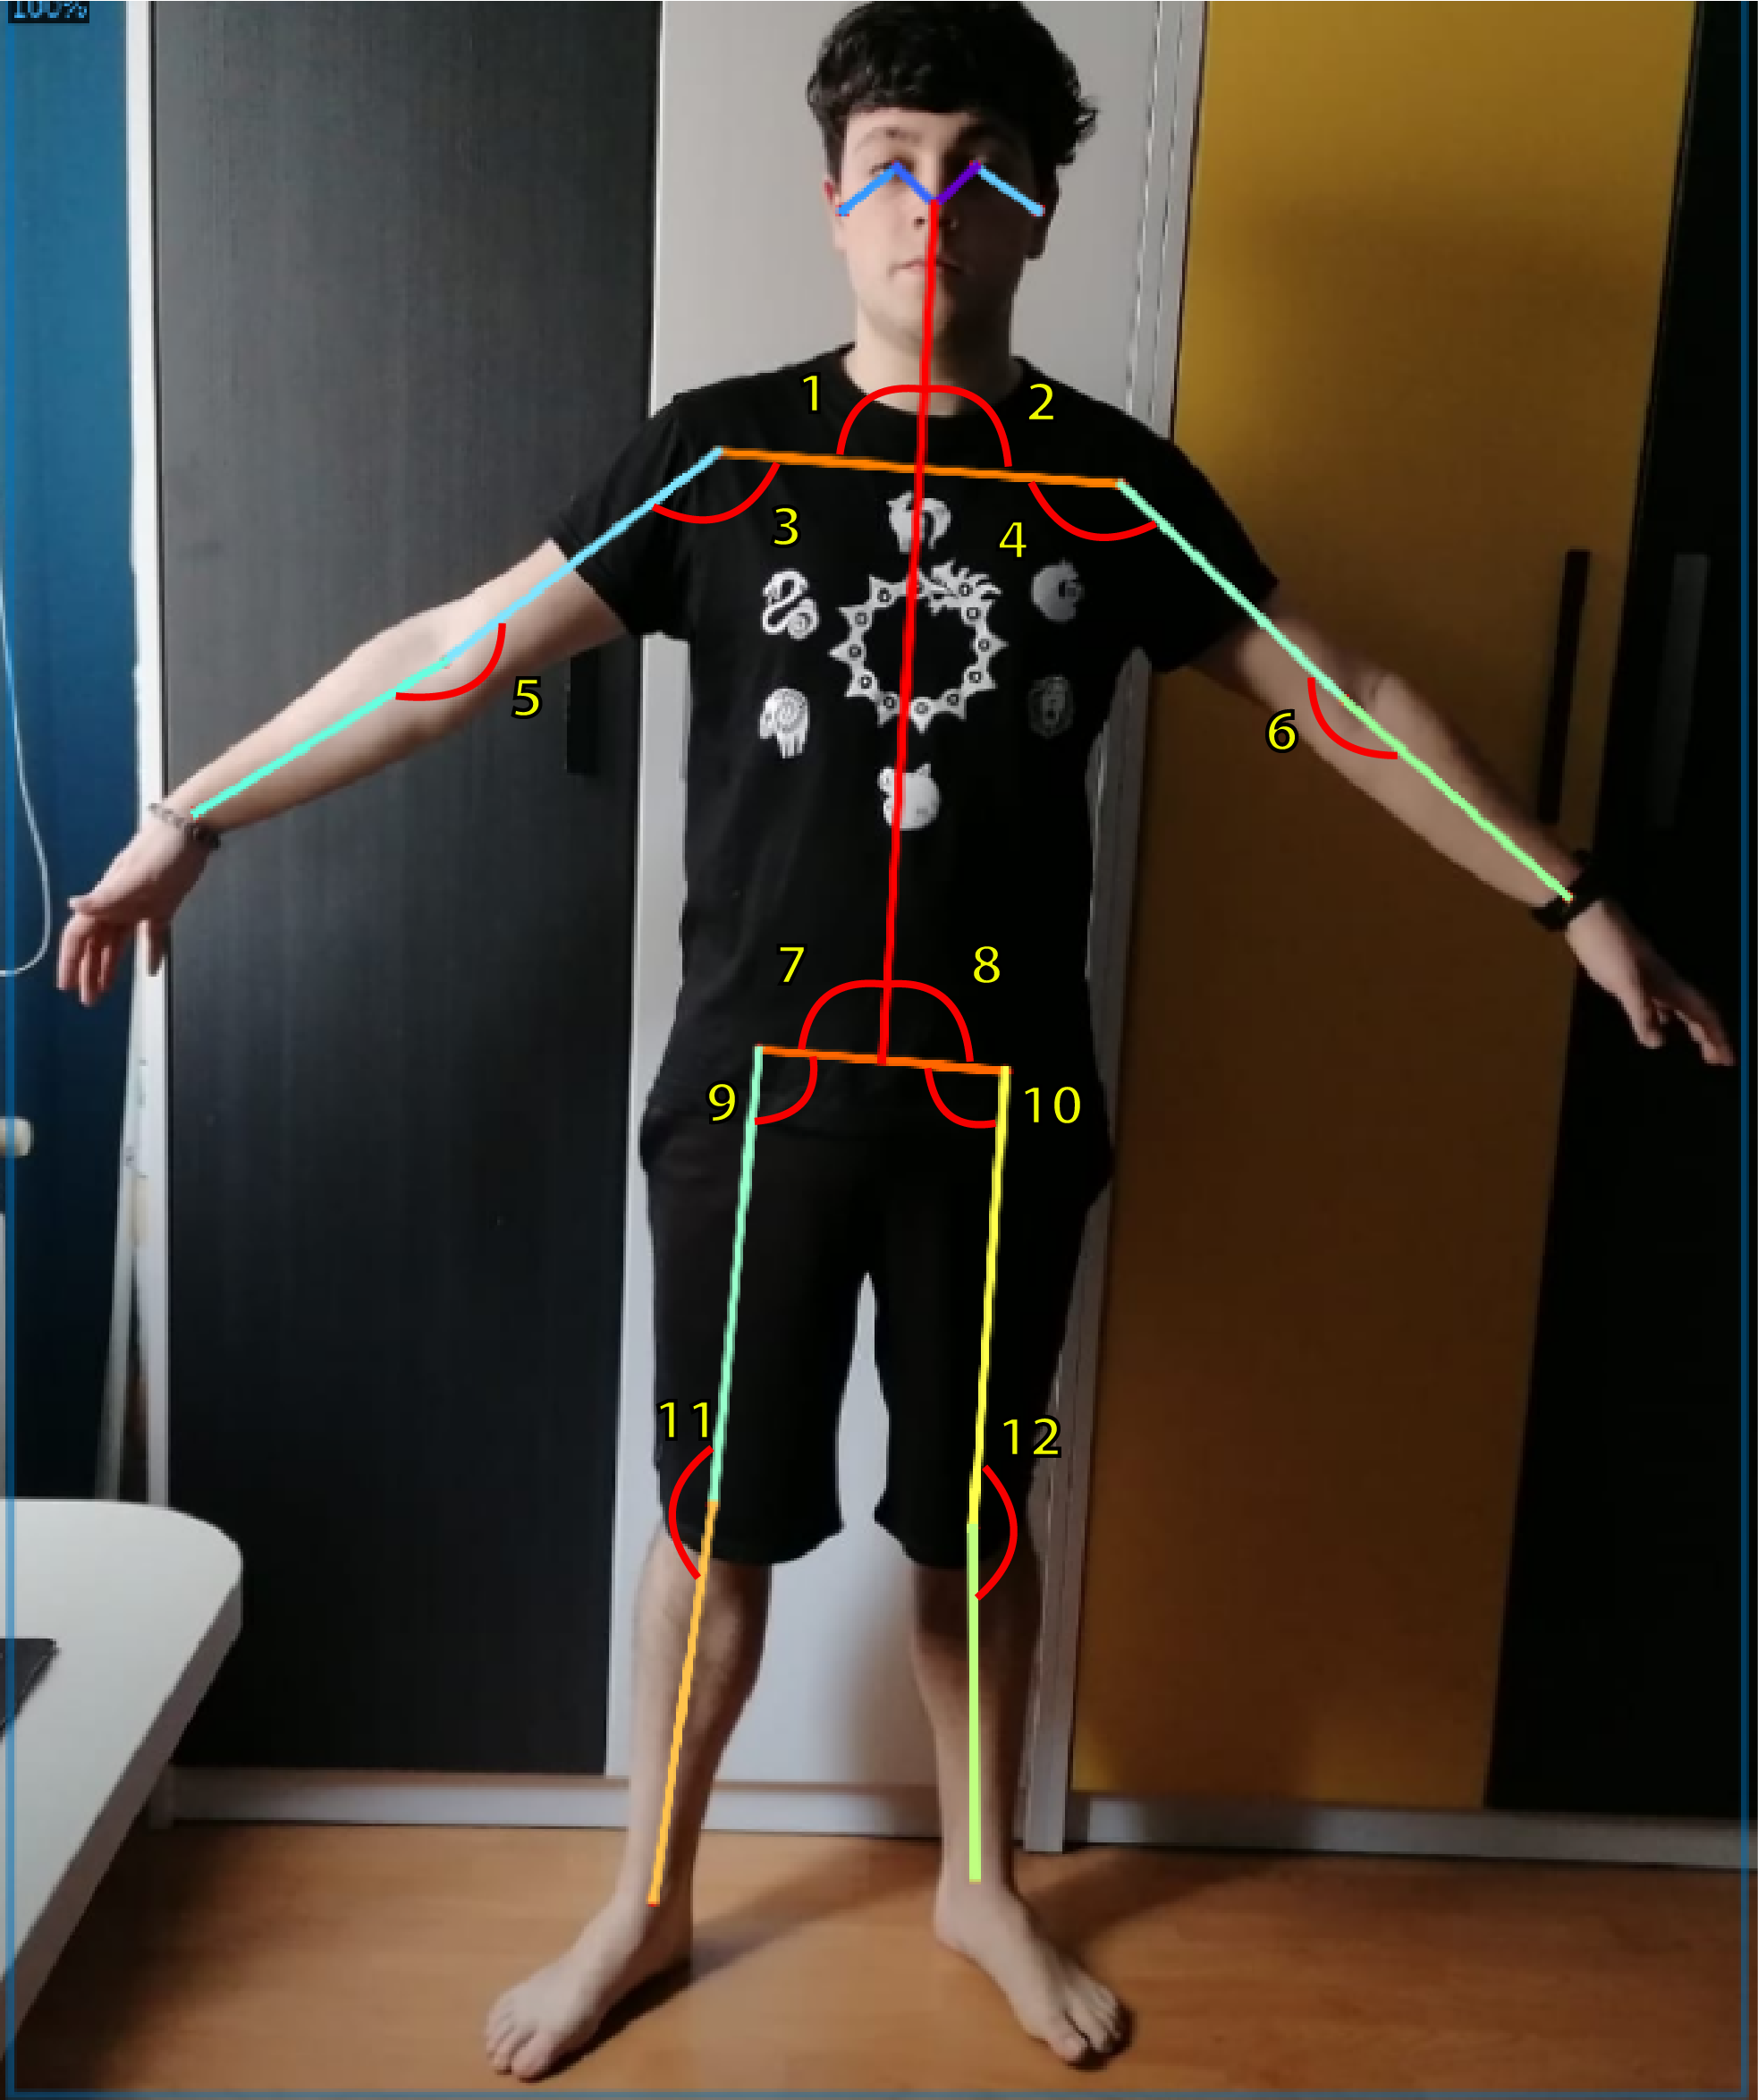
\includegraphics[width=0.5\textwidth]{estiradosAbajo2}
	\caption{Ejemplo ángulos sobre los que se calcula la diferencia entre posiciones.}
	\label{fig:estiradosAbajo2}
\end{figure}

La comparación de cada una de las partes se realiza calculando la suma de los valores absolutos de las restas de los valores de los ángulos entre las dos posiciones.

\subsection{Problema con los ángulos de los brazos}
Tras haber implementado la primera versión, se realizaron unas pruebas para comprobar su funcionamiento. En estas pruebas se encontró un fallo muy importante, ya que los ángulos que se obtenían eran hasta 180 grados, si se superaba este valor el ángulo se calculaba sobre el otro lado del punto central, es decir, nunca es superior a 180 grados. Es por ello que  posiciones como las que se pueden ver en las figuras~\ref{fig:brazosAbajo} y~\ref{fig:brazosArriba} tiene ángulos en ambos codos muy parecidos, aunque sean posiciones casi contrarias.

\begin{figure}[ht]
	\begin{subfigure}{.48\textwidth}
		\centering
		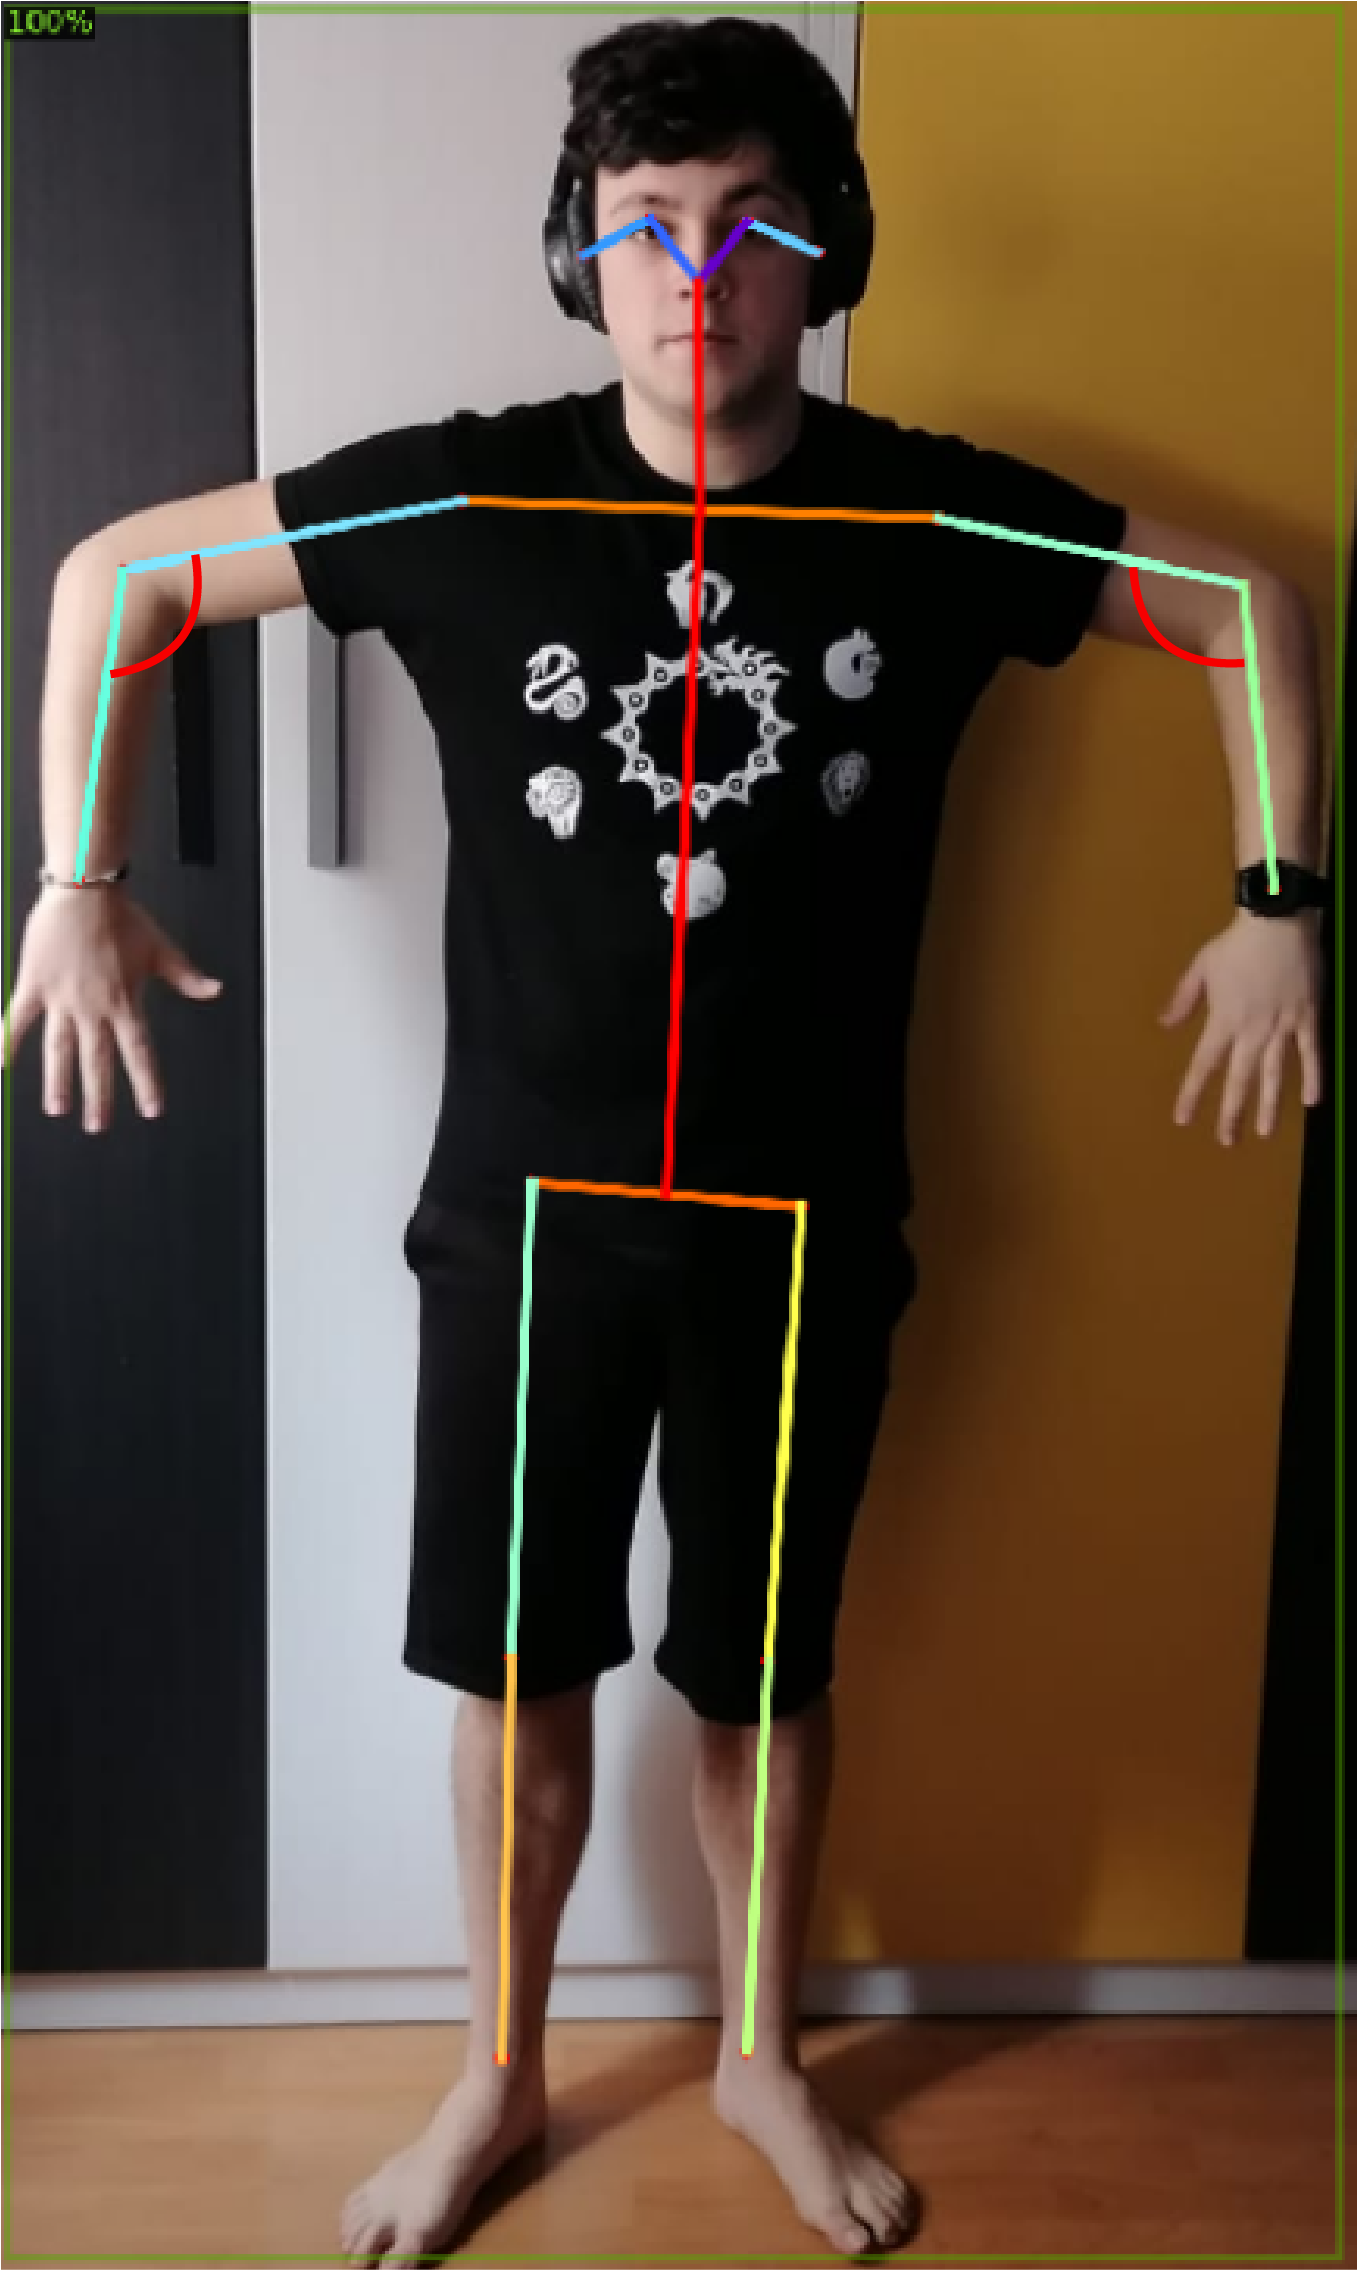
\includegraphics[width=0.5\textwidth]{brazosAbajo}
		\caption{Posición con los codos en 90 grados mirando hacia abajo.}
		\label{fig:brazosAbajo}
	\end{subfigure}
	\begin{subfigure}{.48\textwidth}
		\centering
		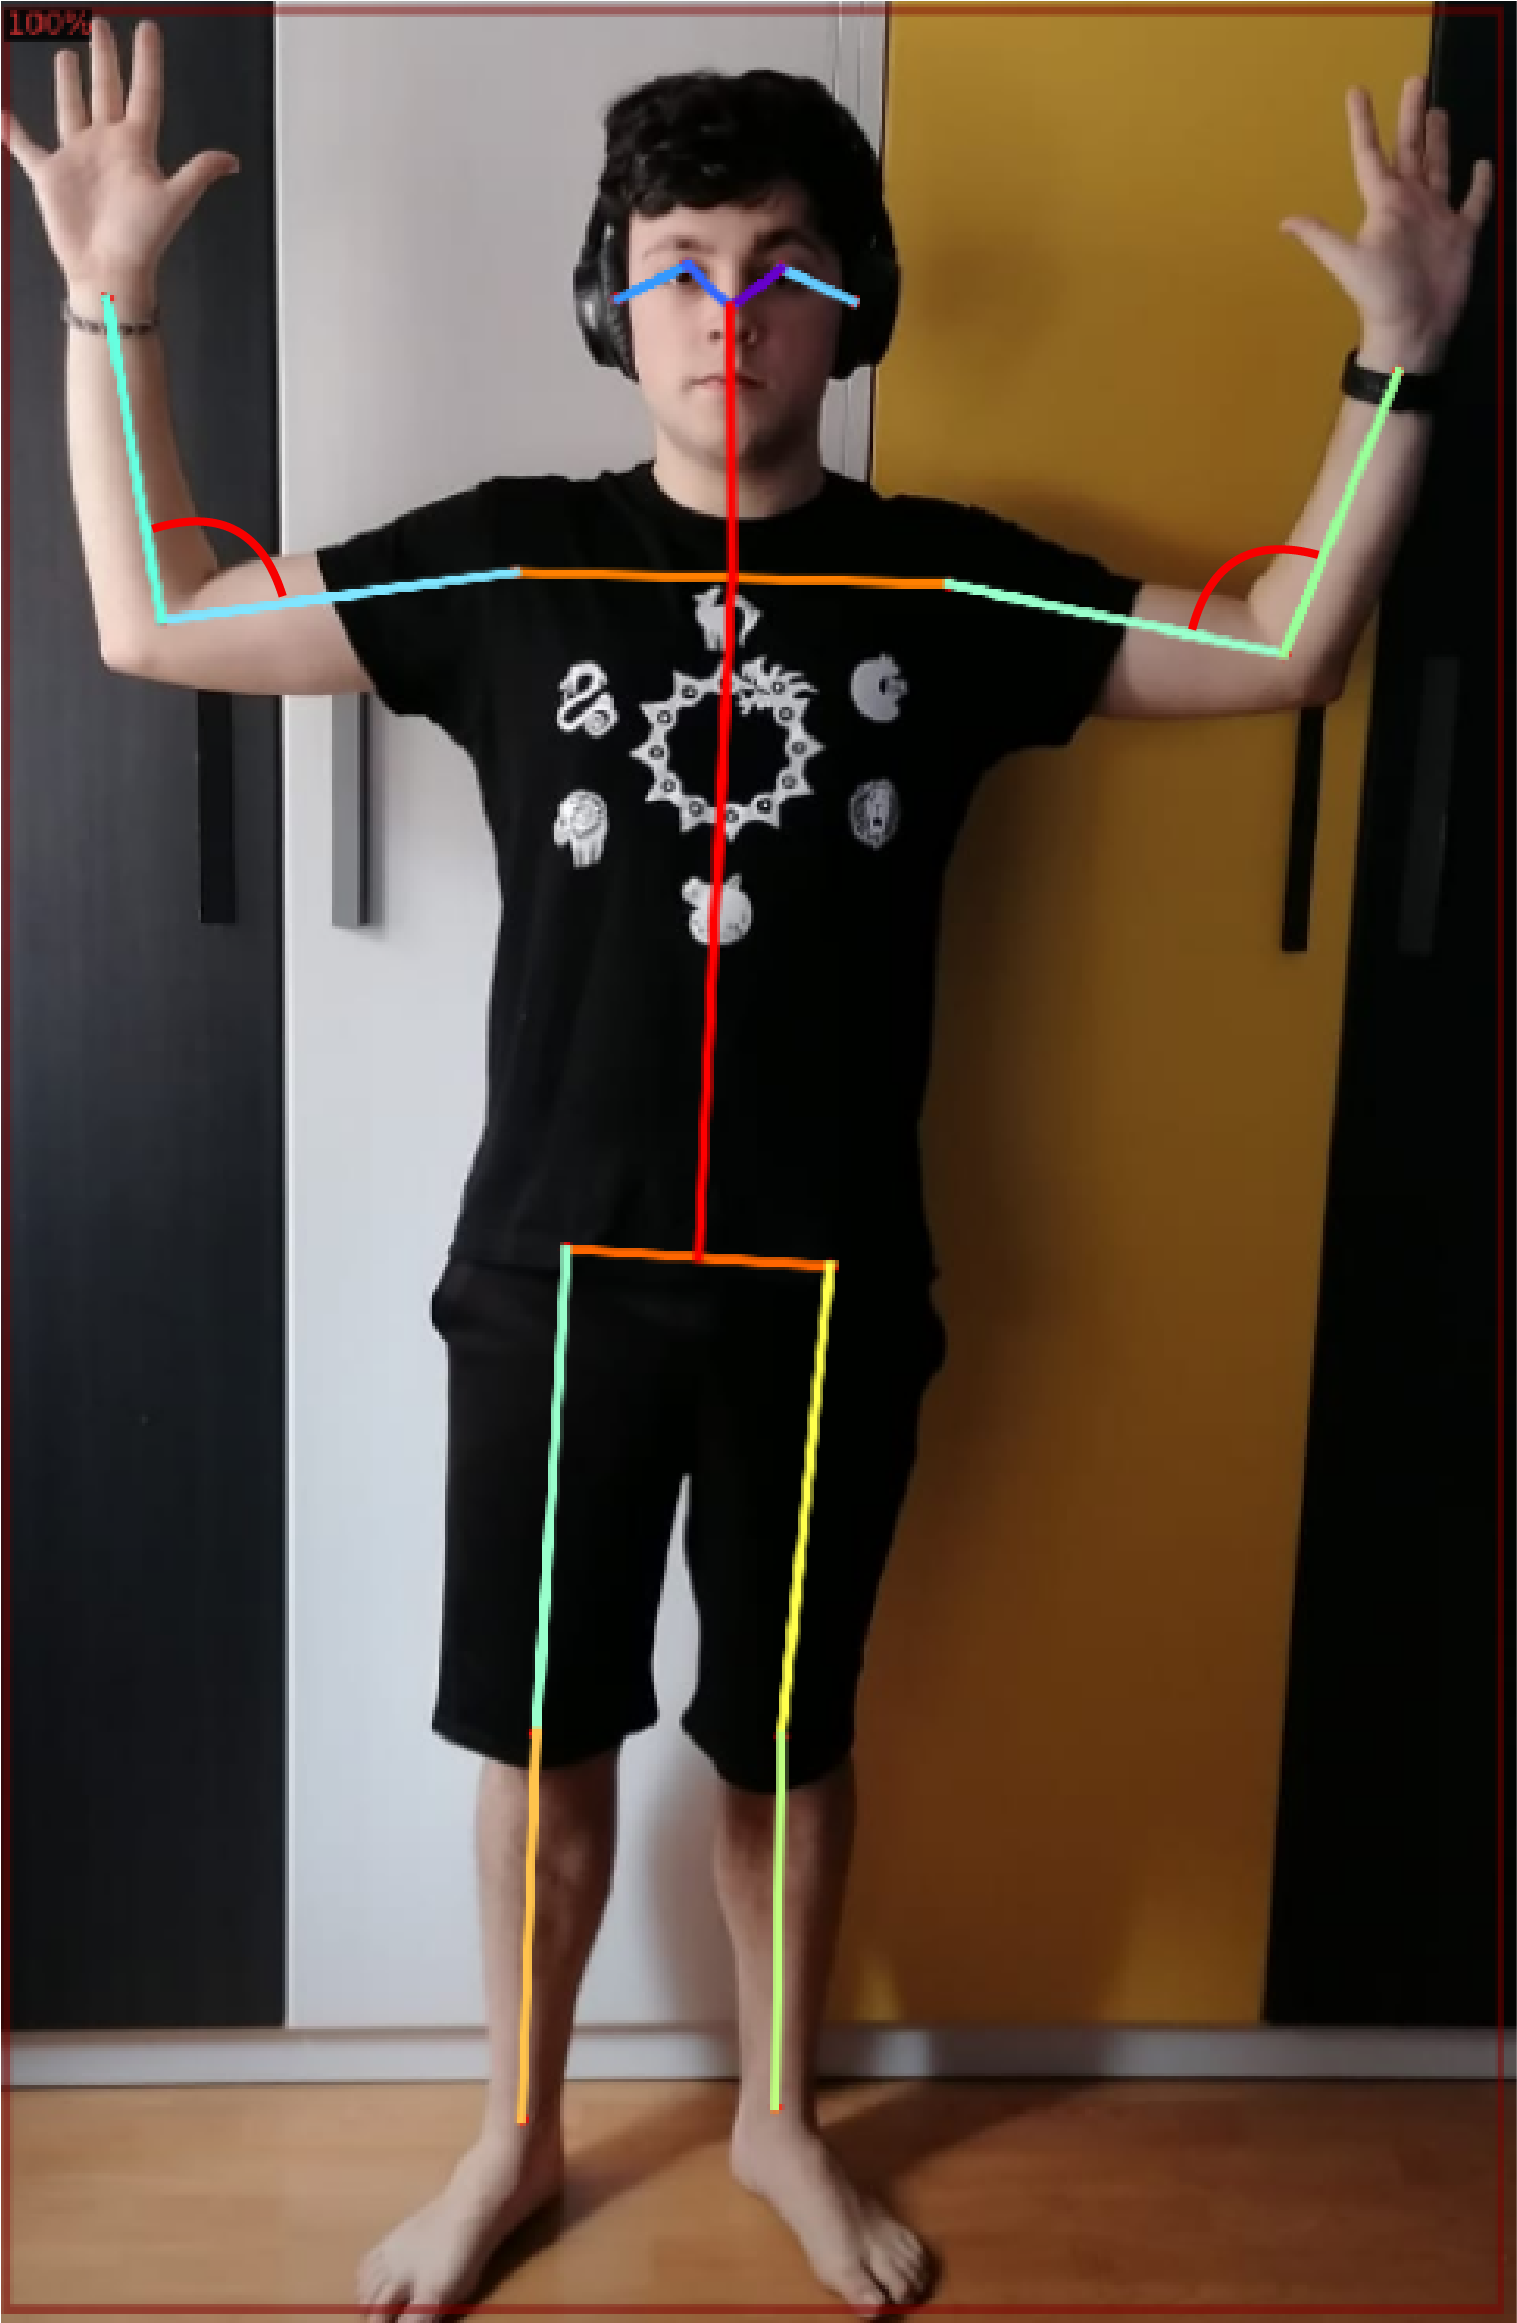
\includegraphics[width=0.55\textwidth]{brazosArriba}
		\caption{Posición con los codos en 90 grados mirando hacia arriba.}
		\label{fig:brazosArriba}
	\end{subfigure}
	\caption{Ejemplos problemas con codos.}
	\label{fig:codos90}
\end{figure}

Este error que se descubrió que pasaba en los codos, se encontró también en la comparación de hombros. Un ejemplo de este error en los hombros se puede ver en las figuras~\ref{fig:estiradosAbajo} y~\ref{fig:estiradosArriba} que obtienen ángulos muy parecidos, aunque sus posiciones sean casi contrarias.


\begin{figure}[ht]
	\begin{subfigure}{.48\textwidth}
		\centering
		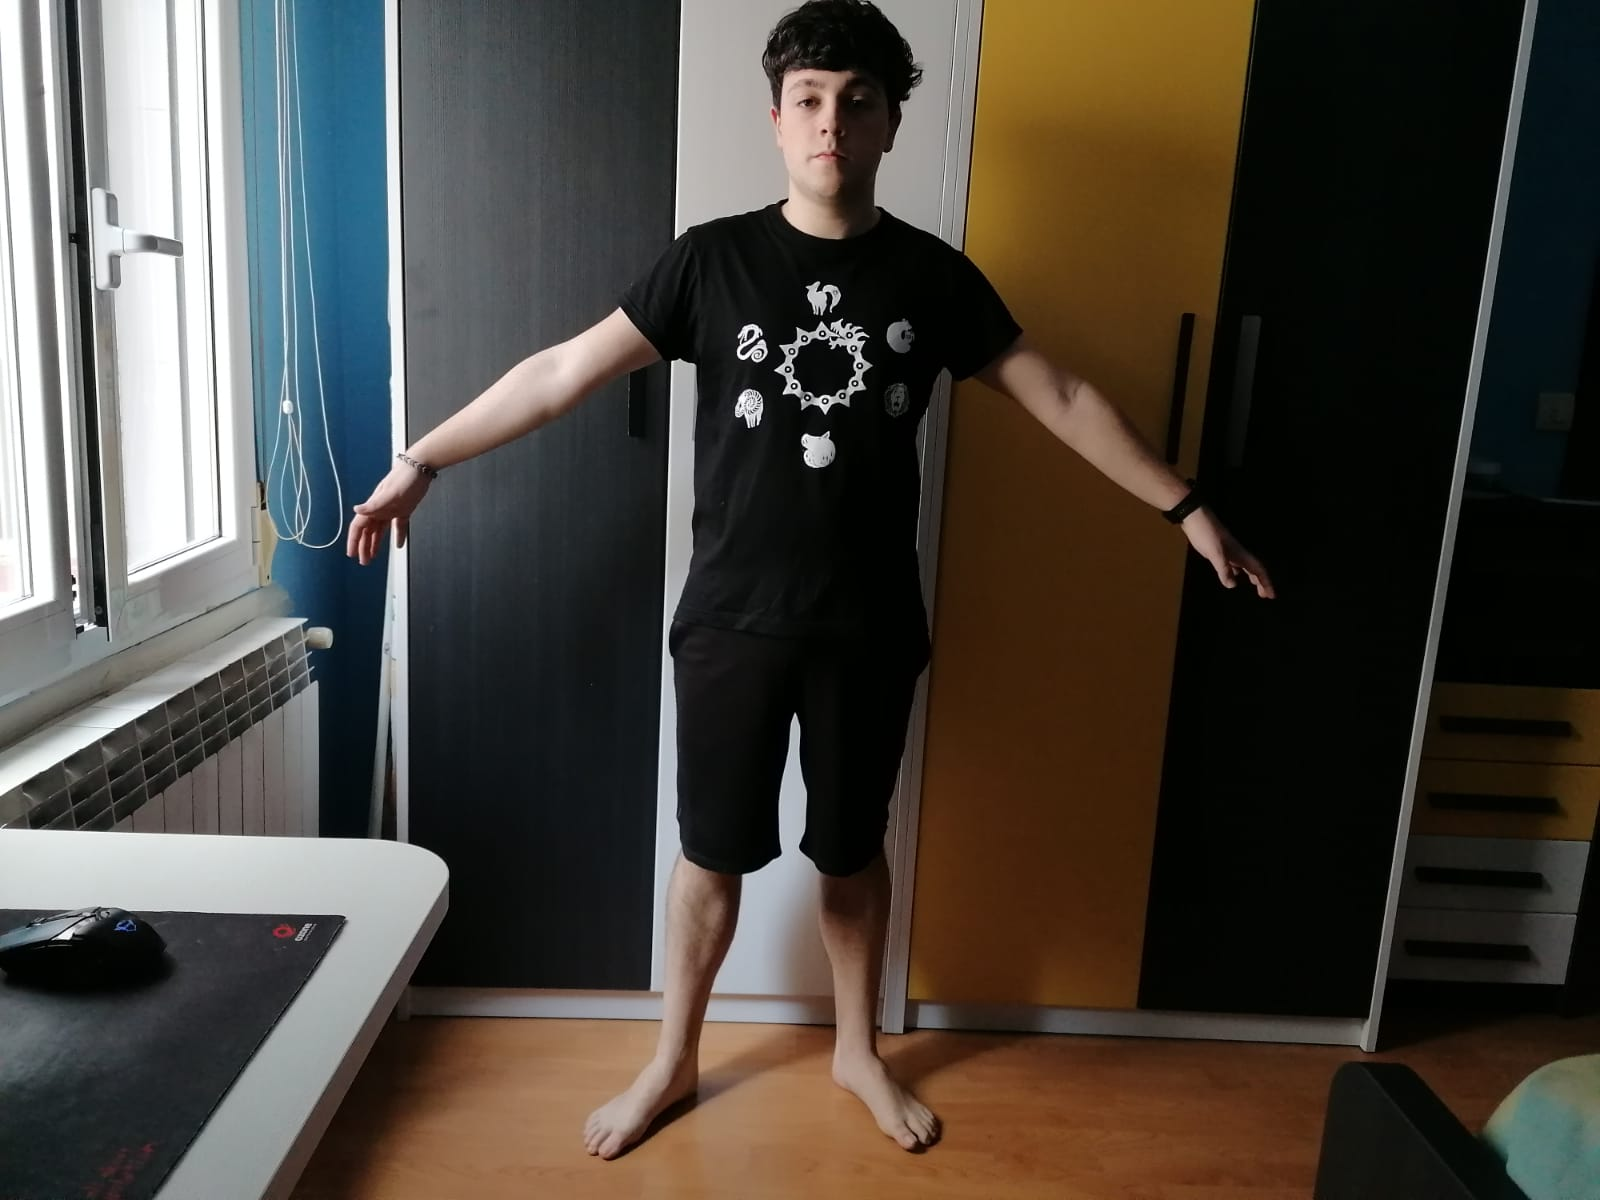
\includegraphics[width=0.7\textwidth]{estiradosAbajo}
		\caption{Posición con los hombros en 45 grados mirando hacia abajo.}
		\label{fig:estiradosAbajo}
	\end{subfigure}
	\begin{subfigure}{.48\textwidth}
		\centering
		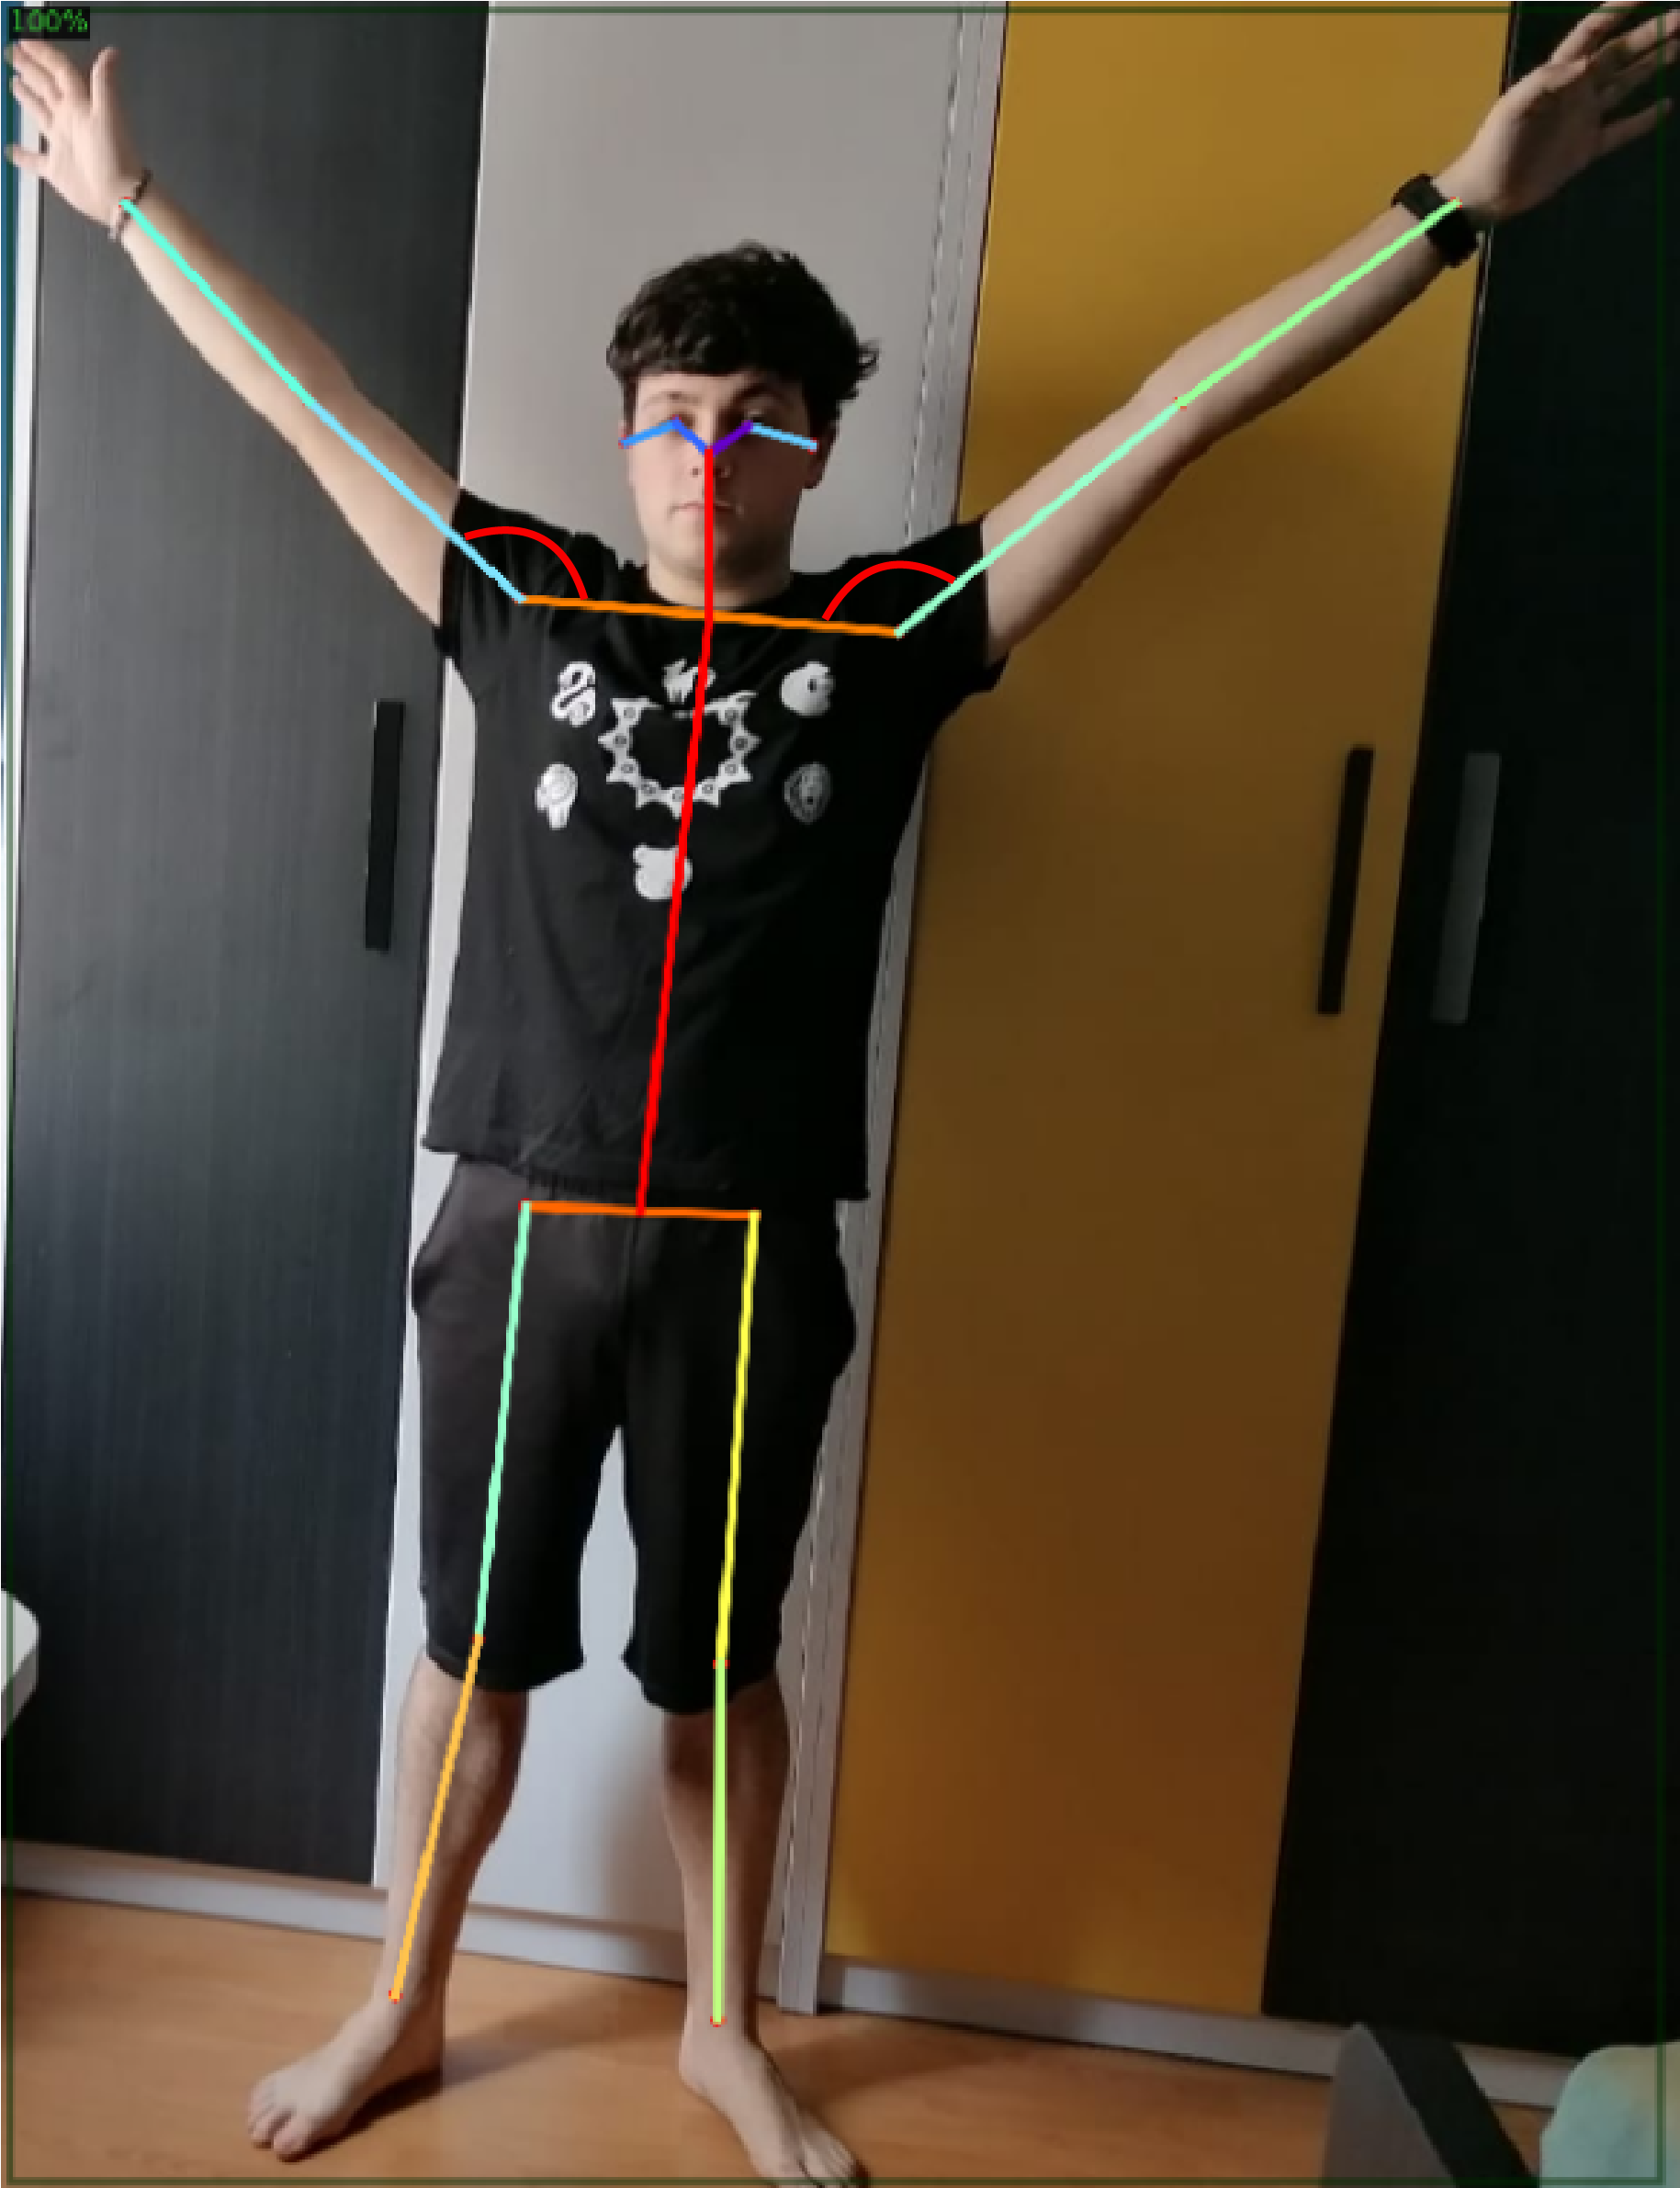
\includegraphics[width=0.65\textwidth]{estiradosArriba}
		\caption{Posición con los hombros en 45 grados mirando hacia arriba.}
		\label{fig:estiradosArriba}
	\end{subfigure}
	\caption{Ejemplos problemas con hombros.}
	\label{fig:hombros90}
\end{figure}

Para poder solucionar estos problemas lo primero que se hizo fue pasar los ángulos de los hombros que se encontraban en la comparación del torso a la comparación de los brazos. Después, para ambas partes se implementó el algoritmo que se puede ver en la figura~\ref{fig:DF_comparacionV2} para poder penalizar estos casos especiales. El algoritmo se recorre por cada una de las zonas y por cada uno de los lados (izquierda y derecha) para ambas posiciones, y se penaliza solo cuando una zona de un lado tiene un tipo de 1 y la correspondiente en la otra zona tiene tipo 2, o viceversa.

\begin{figure}[h]
	\centering
	\includegraphics[width=0.6\textwidth]{DF_comparacionV2}
	\caption{Diagrama de flujos penalización comparación versión 2.}
	\label{fig:DF_comparacionV2}
\end{figure}

Una vez se implementó esta nueva comparación para los brazos, se realizaron una serie de imágenes de prueba para poder confirmar el correcto funcionamiento de la nueva implementación.

\subsection{Umbral y penalización}
Como se ha comentado, en esta segunda versión, que se centró en el problema con los brazos, se han utilizado dos parámetros: un umbral para definir el rango en el que se considera que un ángulo está estirado o no, y la penalización que se aplica si los tipos son distintos.

Al principio se puso un umbral de 10 grados, que para las imágenes de pruebas que se obtuvieron ofrecieran buenos resultados, diferenciando correctamente cuando una de las partes estaba o no estirada. Lo mejor de que este valor sea un parámetro, es que se puede modificar dependiendo del ejercicio a realizar.

Por otro lado, al implementar la penalización se utilizó el mismo valor tanto para los codos como para los hombros, con una valor de 180 grados de penalización. Pero en comprobaciones que se realizaron después, se observó que penalizar a los hombros con el mismo valor que a los codos no era correcto, ya que la diferencia no era tan grande. Es por ello que se dividió este parámetro de penalización en dos, uno para los codos a 180 y otro para los hombros a 90. Aun así, como pasa con el umbral, estos valores se pueden modificar dependiendo del ejercicio a comparar.

\section{Versión 3 de comparación, uso de medias}
Una vez se creía que la comparación de posiciones era correcta había que dar sentido a los valores obtenidos. La forma que se encontró más oportuna para poder realizar esta operación fue el uso de la media de los valores obtenidos en las distintas zonas con las que se trabaja (brazos, piernas y torso).

Además, se implementó el cálculo de la media de tal manera que al aplicar los distintos pesos a las zonas el valor final obtenido siguiese siendo un valor entre 0 y 180 (la distancia máxima que puede haber entre dos ángulos).

Teniendo esto en cuenta, el resultado final se calcula con la siguiente fórmula (siendo $total$ la suma de los tres pesos):
\begin{equation}
\begin{split}
resultado = (pesoBrazos/total)*compBrazos +\\ (pesoPiernas/total)*compPiernas (pesoTorso/total)*compTorso
\end{split}
\end{equation}

\section{Error en brazos, nueva posición y comparación}
En este punto se creía que se tenía una versión final para la comparación de posiciones, pero para probar el funcionamiento de las implementaciones se realizó una nueva prueba sobre los vídeos originales. En esta segunda prueba se encontró un error muy grave, ya que se penalizaban situaciones en los brazos que nunca se deberían de penalizar.

Estos casos donde se penalizaban eran cuando las manos pasaban de estar por encima de los codos a pasar por debajo, o viceversa. Un ejemplo de esta situación se puede ver en la figura~\ref{fig:errorbrazos}, donde la diferencia en los brazos entre las dos imágenes se debería calcular únicamente con la diferencia de los ángulos de los codos, pero que con la implementación de la versión 3, además de la diferencia entre los ángulos, se sumaría una penalización de 180 grados a la diferencia.

\begin{figure}[h]
	\centering
	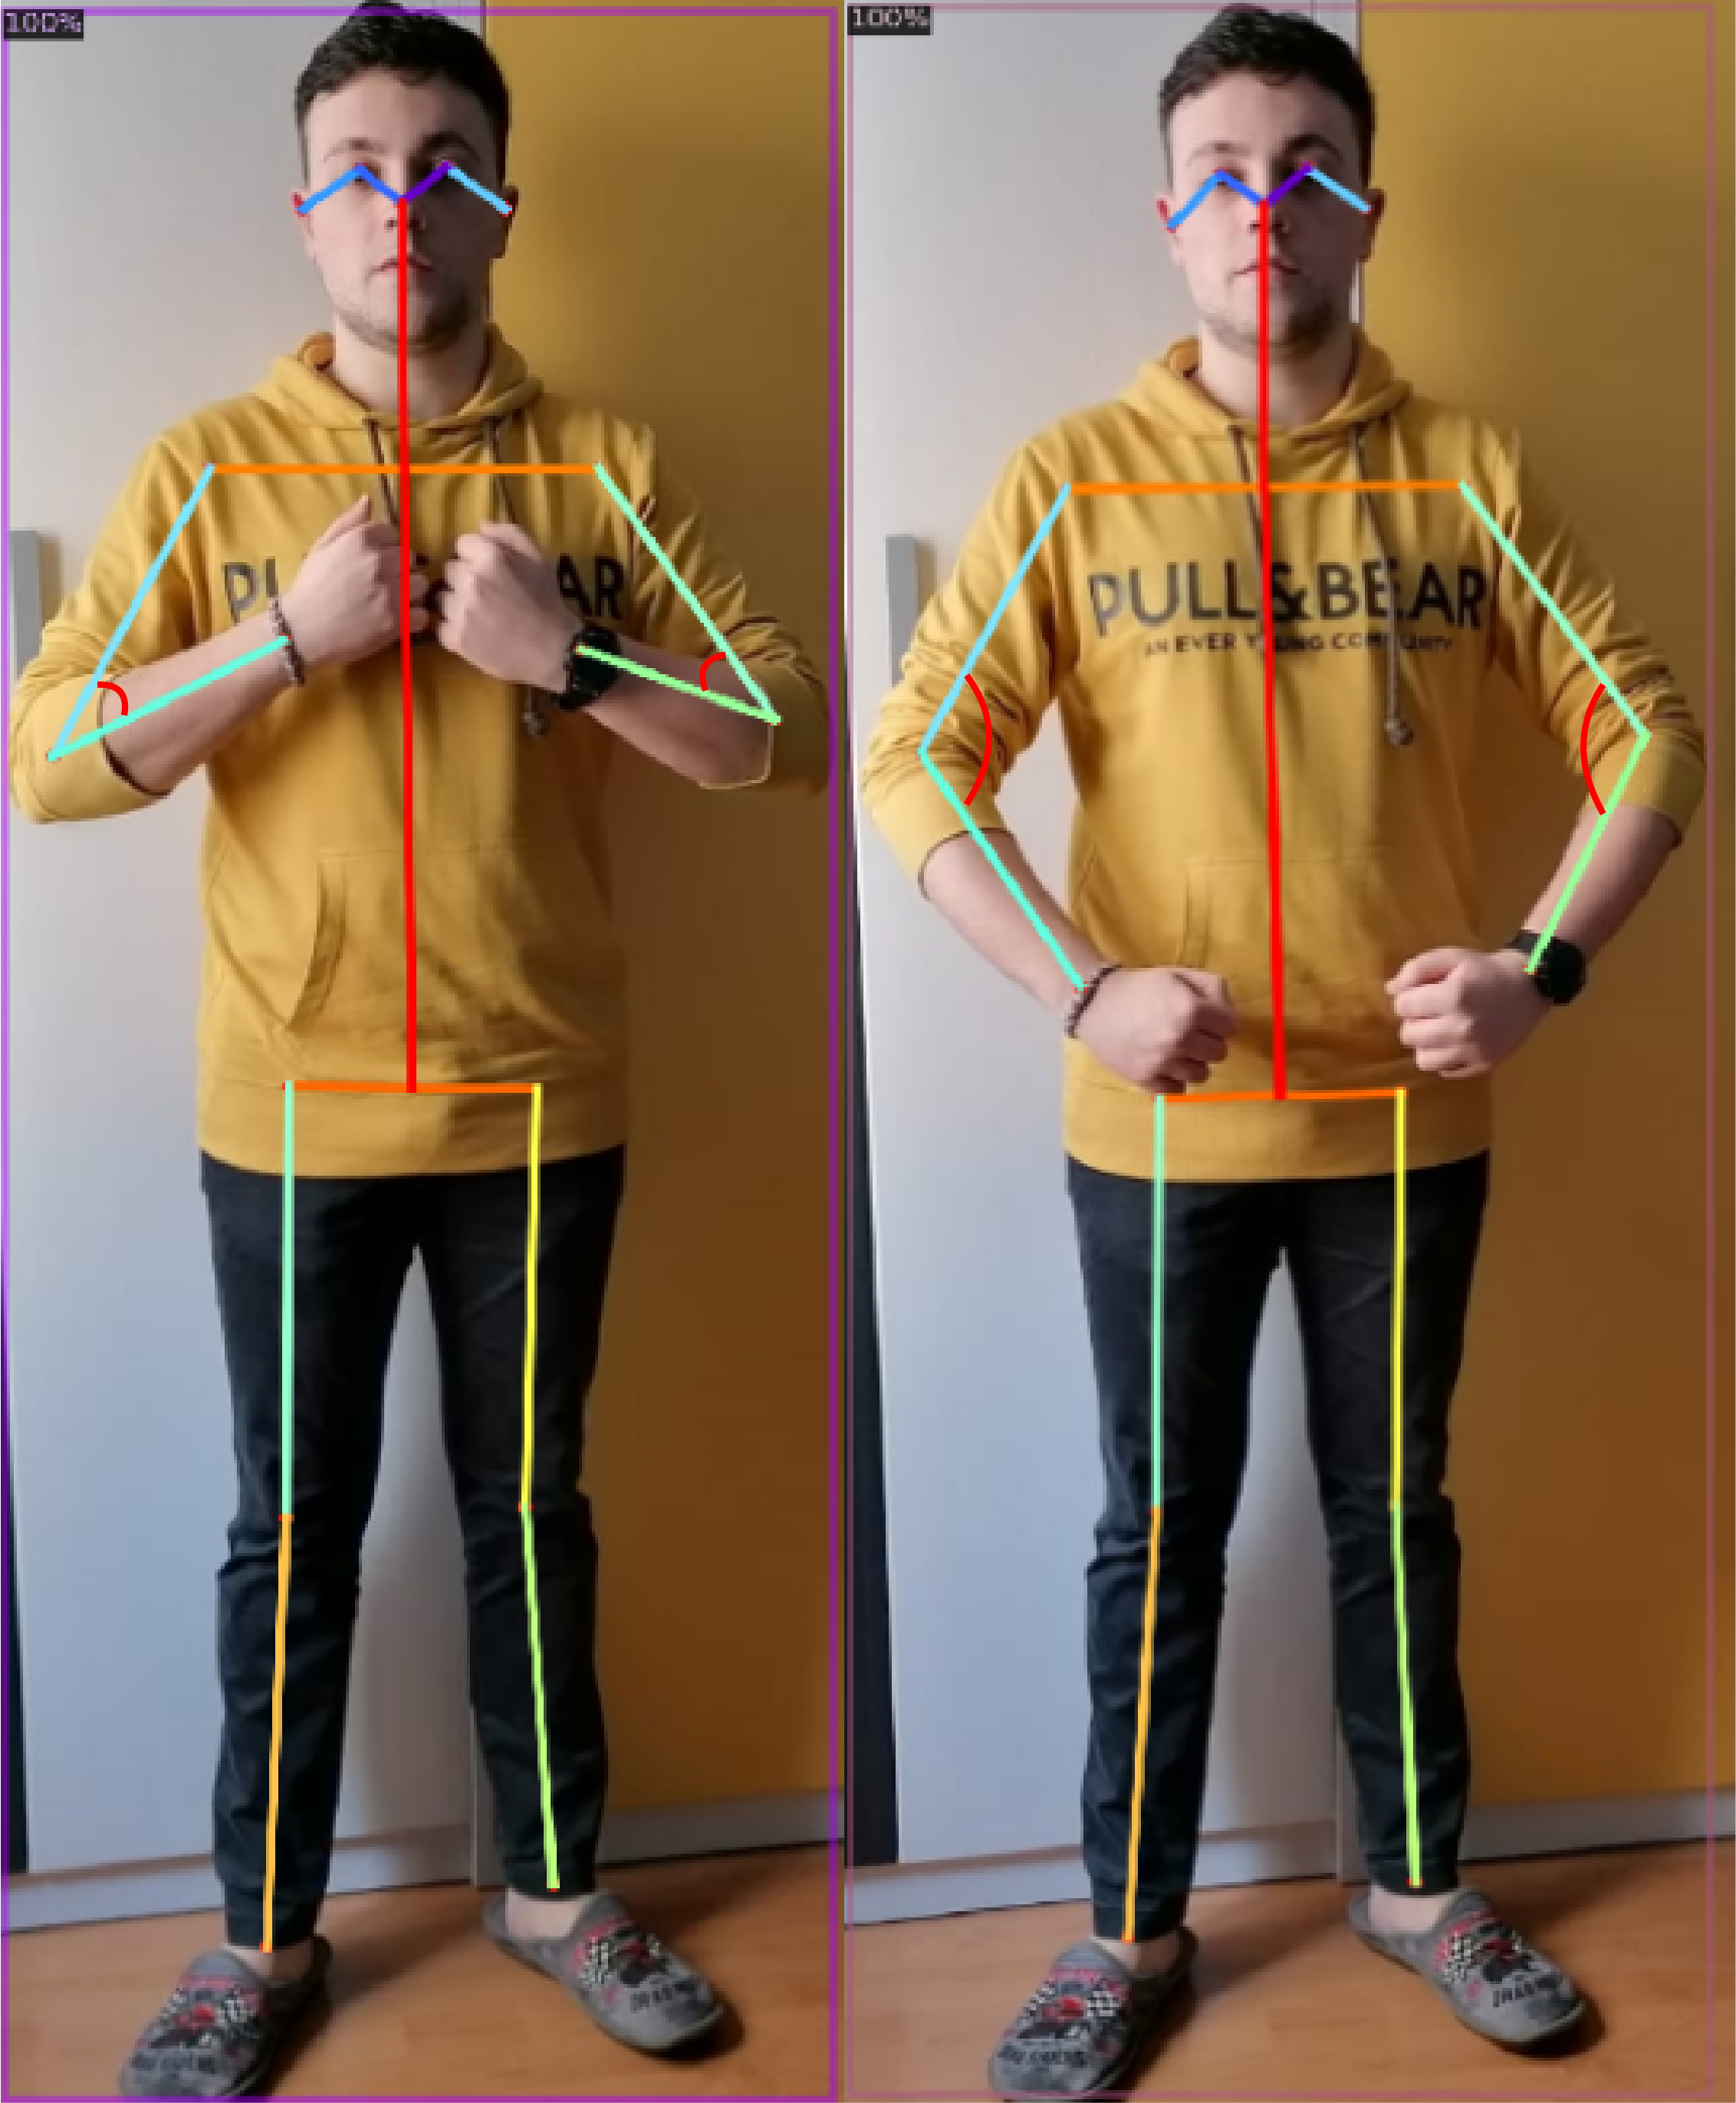
\includegraphics[width=0.5\textwidth]{errorbrazos}
	\caption{Ejemplo de error en la comparación de brazos.}
	\label{fig:errorbrazos}
\end{figure}

Ante dicha situación, se plantearon una serie de posibles soluciones a este problema ya reincidente. Primero se intentó dar solución al problema manteniendo el sistema de la posición y el resto de comparaciones que no daban errores, pero no se ideó una solución plausible que solucionara todos los problemas encontrados en las diversas versiones de la comparación de posiciones. Es por ello que se pasó a hacer una cambio más radical, subiendo a un nivel superior el problema, a la clase de \textit{Python} de la posición.

\subsection{Nueva versión clase posición}

En la primera versión de esta clase, los ángulos se calculaban de forma que nunca eran superiores a 180 grados, lo que daba la necesidad de penalizar ciertas situaciones.

En la segunda versión de la clase se eliminó la condición de que los ángulos fuesen solo de 180 grados (salvo para los ángulos del cuello y de la cadera con el torso, ya que estos ángulos no pueden ser mayores de 180 por fisionomía humana). Para poder expresar el ángulo en un rango de 360 grados se implementó el siguiente algoritmo que utiliza la función anterior de cálculo del ángulo entre 3 puntos:

\begin{algorithm}[H]
	\SetAlgoLined
	\KwData{$P1, P2, P3$ puntos}
	\KwResult{Ángulo en 360 grados }
	ang = calcularAuxAngulo($P1$,$P2$,$P3$)\\
	\eIf{$P1$ y $P2$ a la misma altura (mismo valor en $y$)}{
		\If{P3 en exterior}{
			ang = $360$ - ang\\
		}
	}{
		y = ecuacionDeLaRecta(P1,P2)\\
		\If{El valor de P3 de y es mayor que y}{
				ang = 360 - ang\\
		}
	}
	\textbf{return} ang
	\caption{Cálculo del ángulo en 360 grados.}
\end{algorithm}


Los pasos que sigue este algoritmo son:
\begin{enumerate}
	\item Calcular el ángulo en un rango de 180 grados, con la implementación de la anterior versión de la clase de la posición.
	\item Comprobar si los dos primeros puntos, de los tres estudiados, forman una línea vertical comprobando la resta en sus valores del eje $x$. Si son iguales ir a 3, sino ir a 4.
	\item Si los dos puntos forman una línea vertical no tiene sentido comparar la altura con el tercer punto. Es por ello que lo que se hace es comprobar, dependiendo del lado (izquierda o derecho), la posición del tercer punto analizando si este está más cercano al centro del cuerpo (el ángulo se mantiene igual), o si por el contrario está más al exterior del cuerpo donde se realiza una resta de 360 grados menos el ángulo calculado.
	\item Si por el contrario los dos puntos no están en una línea vertical (caso más común) se calcula la ecuación de la recta con estos dos primeros puntos. En esta ecuación de la recta, se sustituye el valor de $x$ por el valor del eje del tercer punto. Por último, se comprueba si el valor de $y$ calculado con la ecuación de la recta, sustituyendo la $x$ es superior (se mantiene el ángulo) o inferior al valor $y$ del tercer punto donde habría que cambiar el valor del ángulo por 360 menos el ángulo calculado al principio del algoritmo.
	\item Se devuelve el valor calculado del ángulo.
\end{enumerate}

\subsection{Nueva versión comparación}
Una vez se había modificado la clase de la posición, era necesario hacer una serie de cambios en la comparación de éstas. En este caso, al realizar estos cambios, ya no hacía falta <<discriminar>> la comparación de los brazos, ya que ahora todos se calculan de la misma forma y no se necesita ningún umbral ni penalización. Además, aprovechando que no había que realizar ninguna discriminación, por la zona que se estuviese comparando, se realizó una factorización del código implementado para reducir el código repetido.

Para esta cuarta versión de la comparación de las posiciones se realizaron dos funciones. La primera función permite el cálculo de la media de la diferencia entre los ángulos de las zonas pasadas. El pseudocódigo de esta función se puede ver a continuación:

\begin{algorithm}[H]
	\SetAlgoLined
	\KwData{$pos1, pos2$ posiciones; $zonas$}
	\KwResult{Grados de diferencia entre las zonas pasadas}
	partes = [``D'',``I'']\\
	res = 0\\
	\For{i in partes}{
		\For{j in zonas}{
			aux = absoluto diferencia de ángulos pos1 pos2\\
			
			\eIf{aux > 180}{
				res += 360-aux\\
			}{
				res+=aux\\
			}	
		}
	}
	\textbf{return} res/(len(partes)*len(zonas))
	\caption{Cálculo de la diferencia por zona.}
\end{algorithm}

Como se puede ver en el código, esta implementación permite la comparación de todas las zonas de la posición y siempre devuelve una diferencia media entre las zonas comparadas que nunca supera los 180 grados, es decir, siempre devuelve la distancia mínima entre los ángulos.

Pero para poder dar distintos pesos a las distintas zonas a comparar, se implementó la segunda función que llama a la función anterior, \texttt{comparacionZona}. El pseudocódigo de esta función final que devuelve la diferencia media aplicando los pesos se puede ver a continuación:

\begin{algorithm}[H]
	\SetAlgoLined
	\KwData{$pos1, pos2$ posiciones; $pesos$}
	\KwResult{Grados de diferencia y porcentaje de exactitud}
	zonas=\{``brazos'':[``angCodo'',``angHombro''],\\
		``piernas'':[``angRodilla'',``angCadera''],\\
		``torso'':[``angCaderaTorso'',``angCuelloSup'']\}\\
	res = 0\\
	total=0\\
	\For{i in pesos}{
		\If{i no está en las keys de zonas}{\textbf{raise Exception}}
		total+=pesos[i]
	}
	\For{i in zonas}{
		res+=(pesos[i]/total)*comparacionZona(pos1,pos2,zonas[i])
	}

	porcentaje = res*100/180\\
	\textbf{return} res, 100-porcentaje
	\caption{Cálculo de la diferencia de posiciones.}
\end{algorithm}

Como se observa en el código, la implementación recorre las distintas zonas de las cuales calcula la comparación entre las posiciones y le aplica el peso considerado. Además, una vez calculada la diferencia final, al estar entre 0 y 180 grados por utilizar las medias, se calcula el porcentaje inverso de exactitud entre las dos posiciones. Este porcentaje se interpreta como el porcentaje de exactitud entre las posiciones, siendo el 100\% el valor máximo donde las dos posiciones son totalmente iguales.

\section{Comprobación de la última versión}
Una vez se terminaron de implementar estas nuevas versiones, se probaron con las imágenes de la sección~\ref{PrimeraVersion} que la implementación funcionaba correctamente con los datos que las primeras dos versiones tenían grandes problemas. Después, para poder probar el funcionamiento y sobre todo el rendimiento de la implementación, se desarrollaron unas funciones que permiten recorrer todos los vídeos de una carpeta. De cada uno de estos vídeos, la función permite comparar un fotograma con el siguiente de ese mismo vídeo (objetivo principal del proyecto). Cabe comentar en que esta comparación se ha dado el mismo peso a todas las zonas comparadas. Gracias a estas funciones se pudo obtener los siguientes datos de cada uno de los vídeos:
\begin{itemize}
	\item Media de la diferencia de los grados en todo el vídeo.
	\item Diferencia máxima en grados en todo el vídeo.
	\item Diferencia mínima en grados en todo el vídeo.
	\item Desviación típica entre las diferencias de los grados.
	\item Media del porcentaje de exactitud.
	\item Porcentaje máximo de exactitud.
	\item Porcentaje mínimo de exactitud.
	\item Desviación típica de los porcentajes.
	\item Número de fotogramas en el vídeo.
	\item Tiempo de obtención de las posiciones del vídeo.
	\item Tiempo de comparación de las posiciones del vídeo.
	\item Tiempo de cálculo de estadísticas de las comparaciones del vídeo.
	\item Tiempo total.
	\item Tiempo total empleado por fotograma.
\end{itemize}

Los resultados obtenidos en esta fase se pueden ver en:
\begin{itemize}
	\item Resultados diferencia en grados: tabla~\ref{tab:difgra}.
	\item Resultados diferencias en porcentajes: tabla~\ref{tab:difpor}.
	\item Resultados tiempos de ejecución: tabla~\ref{tab:tiempos}.
\end{itemize}

\begin{table}[h]
	\centering
	\resizebox{\columnwidth}{!}{
\begin{tabular}{lrrrr}
	\toprule
	Vídeo &  MediaGrados  &  GradosMáximos &  GradosMínimos &  DesviaciónGrados \\
	\midrule
	depie &     $5.26$ &      $34.89$ &       $0.46$ &          $5.93$ \\
	sentado1 &     $2.68$ &      $26.07$ &       $0.05$ &          $3.01$\\
	sentado2-cruzado &     $2.79$ &      $15.35$ &       $0.40$ &          $1.81$\\
	sentado2-cruzado-480 &     $2.74$ &      $14.59$ &       $0.58$ &          $1.72$\\
	sentado3-caja &     $2.62$ &      $34.32$ &       $0.15$ &          $4.13$\\
	sentado4-remangado &     $2.78$ &      $23.80$ &       $0.22$ &          $2.96$\\
	sentado5-chaqueta-abierta&     $2.96$ &      $17.29$ &       $0.42$ &          $1.94$\\
	sentado6-camiseta &     $2.36$ &       $5.27$ &       $0.32$ &          $0.96$\\
	\bottomrule
\end{tabular}
}
\caption{Tabla con las estadísticas de las diferencias en grados.}
\label{tab:difgra}
\end{table}

\begin{table}[h]
	\centering
	\resizebox{\columnwidth}{!}{
\begin{tabular}{lrrrr}
	\toprule
	Vídeo&  PorcMedio &  PorcMáximo &  PorcMínimo &  DesvPorcentaje\\
	\midrule
	depie&        $97.08$ &         $99.74$ &         $80.61$ &              $3.29$\\
	sentado1 &        $98.51$ &         $99.97$ &         $85.52$ &              $1.67$\\
	sentado2-cruzado &        $98.45$ &         $99.78$ &         $91.47$ &              $1.01$\\
	sentado2-cruzado-480 &       $98.48$ &         $99.68$ &         $91.89$ &              $0.95$\\
	sentado3-caja &        $98.54$ &         $99.92$ &         $80.93$ &              $2.29$\\
	sentado4-remangado &       $98.46$ &         $99.88$ &         $86.78$ &              $1.65$\\
	sentado5-chaqueta-abierta &        $98.35$ &         $99.76$ &         $90.39$ &              $1.08$\\
	sentado6-camiseta &        $98.69$ &         $99.82$ &         $97.07$ &              $0.53$\\
	\bottomrule
\end{tabular}
}
\caption{Tabla con las estadísticas de las diferencias en porcentajes de exactitud.}
\label{tab:difpor}
\end{table}

\begin{table}[h]
	\centering
	\resizebox{\columnwidth}{!}{
		\begin{tabular}{lrrrrrr}
	\toprule
	Vídeo&  NFrames &  TiempoObtPos (ms) &  TiempoComp (ms) &  TiempoEst (ms) &  TiempoTotal (ms) &  Tiempo/Frame (ms) \\
	\midrule
	depie&$258$ &          $26735.74$ &           $50.47$ &            $0.21$ &    $26786.42$ &      $103.82$ \\
	sentado1&$445$ &          $50953.61$ &         $80.24$ &            $0.16$ &  $51034.02$ &    $114.68$ \\
	sentado2-cruzado&$286$ &         $32914.02$ &          $44.59$ &            $0.13$ &  $32958.74$ &    $115.24$ \\
	sentado2-cruzado-480&$286$ &          $31126.15$ &          $44.60$ &            $0.12$ &  $31170.87$ &    $108.99$ \\
	sentado3-caja&$299$ &          $33129.63$ &          $46.43$ &            $0.13$ &  $33176.18$ &    $110.96$ \\
	sentado4-remangado&$219$ &         $24638.31$ &          $34.36$ &            $0.11$ &  $24672.78$ &    $112.66$ \\
	sentado5-chaqueta-abierta&$281$ &         $31442.28$ &          $44.33$ &            $0.12$ &  $31486.73$ &    $112.05$ \\
	sentado6-camiseta&$194$ &          $21334.31$ &          $31.36$ &            $0.11$ &  $21365.78$ &    $110.13$ \\
	\bottomrule
\end{tabular}
}
\caption{Tabla con los tiempos de la ejecución.}
\label{tab:tiempos}
\end{table}

Como se puede observar, los resultados comparando los fotogramas de un mismo vídeo dan muy buenos resultados, con medias de porcentaje de exactitud que no bajan del $97\%$, lo que significa que ninguna comparación tiene una media superior a $5.4^{\circ}$ de diferencia.

Si se observan los porcentajes máximos de exactitud y los grados mínimos de diferencia, se observan valores muy positivos, siendo los porcentajes muy cercanos al $100\%$ y los grados muy similares a $0^{\circ}$. Este resultado es el que cabría de esperar, ya que en todo el vídeo es muy probable que haya al menos dos fotogramas contiguos que se difieran muy poco al no haber casi movimiento.

Otro dato importante, que principalmente puede servir para detectar fallos en la posición obtenida por la red neuronal, es el porcentaje mínimo de exactitud y el correspondiente grado máximo de diferencia. Observando estos datos, se puede ver como los grados máximos de diferencia entre dos fotogramas de todos los vídeos es de unos $35^{\circ}$ (que ocurren en el vídeo donde se está de pie). Tras observar en qué fotogramas se haya este máximo, se vio como este valor se debía a un pequeño fallo en la detección de la posición por parte de la red neuronal. Pero este <<problema>> no es importante, debido a que este tipo de movimientos no se realizan en los ejercicios de ejemplos de las rehabilitaciones reales a personas con \textit{Parkinson}, y a que no afecta en gran medida (debido al gran número de fotogramas) a las otras estadísticas, sobre todo a la más importante, la media.

Por último, tras haber comprobado que los algoritmos daban unos resultados bastante positivos, se analizaron los tiempos de ejecución, ya que no hay que olvidarse que este proyecto forma parte de una aplicación más grande que se realizará junto al trabajo de José Luis Garrido Labrador, para poder realizar estas operaciones en un flujo de imágenes. Es por ello que los algoritmos, además de usar la mínima capacidad de memoria posible, debían de ser rápidos. Este tipo de estudios ya se habían realizado en fases anteriores del proyecto, como el estudio  para obtener el mejor modelo de red neuronal que proporcionase los mejores resultados en el menor tiempo posible. En este estudio había que comprobar el tiempo de ejecución de todo el proceso, es decir,  el cálculo de la posición a partir de la salida de la red neuronal, después la comparación de las posiciones obtenidas y por último el cálculo de estadísticas que permitan obtener un resultado legible y comprensible.

Observando los tiempos de ejecución, tabla~\ref{tab:tiempos}, se puede ver como, sin lugar a duda, la ejecución del modelo de la red neuronal y el posterior cálculo de la posición es donde se invierte más tiempo (aun teniendo el modelo ya cargado en memoria como se haría en el despliegue final con la estructura de flujos del compañero). Si se analizan el resto de tiempos, se puede ver cómo la implementación de la comparación de posiciones es muy óptima, siendo el tiempo invertido en esta tarea en el vídeo más largo tan solo de $80.24$ milisegundos. Por último, el calculo de estadísticas sobre las comparaciones realizadas también es muy rápida, no superando en ninguno de los vídeos los $0.22$ milisegundos.

Cabe destacar las diferencias que existen entre los dos vídeos iguales pero con distinta calidad, sentado2-cruzado (720p) y sentado2-cruzado-480 (480p). Como se puede ver en la tabla~\ref{tab:tiempos}, la diferencia entre ambas ejecuciones difiere en poco más de 1 segundo, que como era de esperar se encuentra en la diferencia en las fases de obtención de la posición a partir de la red neuronal y la clase implementada. Si se observan los resultados de la comparación de los vídeos, en las tablas~\ref{tab:difgra} y~\ref{tab:difpor}, se observa que apenas hay diferencias entre las dos ejecuciones. Teniendo esto en cuenta, se puede asegurar que la reducción de calidad de los vídeos mejora el rendimiento de la herramienta manteniendo unos resultados correctos, al menos si la calidad mínima es 480p.

Como se ha comentado, tras realizar todas la pruebas, se concluyó en que estas versiones del cálculo de posición y de comparación de posiciones serían las implementaciones prácticamente definitivas. Es por ello que interesaba saber el tiempo total invertido para realizar el proceso de obtener la posición de un fotograma, comparar esta posición con la siguiente y obtener las estadísticas de esta comparación. Como se puede ver en la tabla~\ref{tab:tiempos}, el tiempo medio de procesamiento de cada fotograma es de $111.07$ milisegundos, un resultado muy bueno si se tiene en cuenta todo el proceso que lleva detrás.

\section{Versión reducida} \label{reducida}
Tras tener la versión final implementada, se vio necesario la reducción de la clase de la posición para poder ahorrar el mayor tiempo y el mayor uso de memoria posible, objetivo esencial al trabajar con un flujo de datos. Una vez se <<limpió>> la clase para obtener la versión reducida, se ejecutaron las pruebas implementadas para la versión anterior para poder observar la mejoría en el tiempo, ya que la salida no se ve afectada (porque solo se eliminaron los cálculos que no se utilizaban en la comparación de posiciones). Los nuevos tiempos de ejecución se puede ver en la tabla~\ref{tab:tiempos2}.

\begin{table}[h]
	\centering
	\resizebox{\columnwidth}{!}{
		\begin{tabular}{lrrrrrr}
			\toprule
			Vídeo&  NFrames &  TiempoObtPos (ms) &  TiempoComp (ms) &  TiempoEst (ms) &  TiempoTotal (ms) &  Tiempo/Frame (ms) \\
			\midrule
			depie&$258$ &          $26605.28$ &          $42.20$ &            $0.17$ &  $26647.66$ &    $104.50$ \\
			sentado1&$445$ &          $50694.96$ &          $73.0$ &            $0.16$ &  $50768.12$ &    $114.34$ \\
			sentado2-cruzado&$286$ &         $32808.08$ &          $37.25$ &            $0.12$ &  $32845.46$ &    $116.06$ \\
			sentado2-cruzado-480&$286$ &          $30906.14$ &          $36.88$ &            $0.11$ &  $30943.13$ &    $109.73$ \\
			sentado3-caja&$299$ &          $32520.80$ &          $38.96$ &            $0.11$ &  $32559.87$ &    $111.89$ \\
			sentado4-remangado&$219$ &         $23845.32$ &          $28.89$ &            $0.10$ &  $23874.31$ &    $109.02$ \\
			sentado5-chaqueta-abierta&$281$ &         $30808.18$ &          $37.17$ &            $0.12$ &  $30845.47$ &    $109.77$ \\
			sentado6-camiseta&$194$ &          $21045.52$ &          $26.34$ &            $0.10$ &  $21071.96$ &    $108.62$ \\
			\bottomrule
		\end{tabular}
	}
	\caption{Tabla con los tiempos de la ejecución con la versión reducida de la posición.}
	\label{tab:tiempos2}
\end{table}

Como se puede observar, la diferencia de tiempos apenas se ha visto afectada, reduciéndose solo un poco en el tiempo de obtención de la posición. El nuevo tiempo medio por fotograma es $110.49$ milisegundos, lo que significa una mejoría de $0.58$ milisegundos. Esta mejoría, al menos a primera vista, no parece significativa, pero teniendo en cuenta que se trabaja con flujos, de muchos datos y muy pesados, cualquier mejora es bien recibida. Además, hay que recordar que esta mejoría en el tiempo de ejecución va acompañada de una mejora en la memoria usada, ya que se necesita prácticamente la mitad de memoria para almacenar las variables de la posición comparado con las versiones anteriores. 

\section{Preparación para flujos}
Tras obtener las versiones definitivas de las implementaciones desarrolladas durante el proyecto, el siguiente paso consistió en pasar todas las implementaciones a un sistema de ficheros \textit{Python} (ya que antes se encontraban en \textit{Jupyter Notebook}), creando así una biblioteca de versiones (carpeta \texttt{/src/python-flujo}).

\section{Integración en el flujo}
Esta fue una de las fases más importantes, ya que se trataba de unir los dos trabajos: el realizado por el compañero, José Luis Garrido Labrador, implementando un flujo de vídeos extensible para poder trabajar con él y este trabajo centrado en el análisis y estudio de las posiciones mostradas en los vídeos.

El primer paso que se realizó fue la explicación de cada uno de los trabajos para poder conocer en qué punto se estaba dentro del proyecto. Una vez se conocía el trabajo realizado por cada uno, se pasó a la implementación de la clase \texttt{Interfaz} en donde se encuentran todos los métodos necesarios para a partir de una imagen recogida del flujo se pueda:
\begin{itemize}
	\item Cargar el modelo parametrizando el \textit{threshold} o sensibilidad en la detección de la persona.
	\item Obtención de la predicción de la posición.
	\item Cálculo de la posición.
	\item Comparación de posiciones.
\end{itemize}

Tras haber implementado esta clase, se pasó a la instalación de la herramienta \textit{Detectron2} en el ordenador personal del compañero donde se encontraba desplegado el flujo para realizar pruebas. Después de haber instalado la herramienta se probó el funcionamiento del flujo con la obtención de la posición, en esta prueba se obtuvo un error debido a que \textit{CUDA} no disponía de la memoria necesaria. Para resolver este problema se implementó una función, que se ejecuta después de calcular la posición de la persona de una imagen, que permite liberar la memoria de \textit{CUDA}. Aún con esta solución, la memoria de la tarjeta gráfica del ordenador personal del compañero no fue suficiente, por lo que se pasó a desplegar el flujo en la estación de trabajo \textit{Gamma}.

Una vez se realizó la instalación de todas las librerías y herramientas necesarias, se desplegó el flujo. En éste se pudo observar el correcto funcionamiento de ambas partes del proyecto, aunque se encontraron los siguientes problemas:
\begin{itemize}
	\item Pérdida de fotogramas en el flujo, que se entendieron como fotogramas en donde la herramienta no había conseguido encontrar los puntos necesarios o simplemente fotogramas perdidos en el flujo.
	\item Tiempo de ejecución algo elevado, debido a la necesidad de cargar el modelo de la red neuronal por cada fotograma a predecir. El problema de la carga continua del modelo se debe a cómo está implementado el flujo del compañero, ya que los que realizan las ejecuciones son \textit{workers} que se crean y se destruyen, por lo tanto cada vez que nace un \textit{worker} ha de cargar el modelo de la red neuronal para poder estimar la posición y realizar los distintos cálculos.
\end{itemize}

Cabe destacar que el tiempo de ejecución en un entorno más realista, es decir, sin tener ni que imprimir ni que almacenar la imagen procesada obtiene una mejora sustancial en el tiempo de ejecución. Es por ello que se implementaron 4 modos de ejecución del flujo:
\begin{itemize}
	\item \textbf{Modo 0}: modo en el que solo se calcula la posición sin necesidad de imprimir ni almacenar el esqueleto. Es el modo más rápido y que más se asemeja al objetivo del proyecto.
	\item \textbf{Modo 1}: modo en el que aparte de devolverse la posición calculada se imprime el esqueleto en la imagen original.
	\item \textbf{Modo 2}: modo en el que aparte de devolverse la posición calculada se imprime el esqueleto en un fondo blanco.
	\item \textbf{Modo 3:} modo en el que aparte de devolverse la posición calculada se imprime el esqueleto en un fondo negro.
\end{itemize}

\section{Estudio final del flujo}
Una vez se había comprobado que la fusión de ambos proyectos era factible y funcionaba correctamente, se realizó un estudio final del flujo paralelizable, para conocer el número de \textit{workers} teóricamente necesarios por cada una de las colas para poder soportar un flujo y una evaluación en tiempo real.

Para ello se realizaron cuatro configuraciones sobre todos los vídeos de pruebas disponibles (un total de 16 vídeos), una en la que se ejecutaba solo la corrección de la imagen y la anonimización de la persona, una segunda donde solo se carga la imagen pero no se realiza ninguna acción (sobre estas dos primeras ejecuciones no se van a comentar nada debido a que es trabajo del compañero), una tercera configuración donde solo se ejecuta el cálculo de la posición de las imágenes y la comparación de las posiciones obtenidas y, por último, una configuración donde se comprobó la ejecución de todas las partes. Además, de cada una de estas configuraciones se realizaron dos ejecuciones, una con el modo 0 donde no se almacenaba la imagen, y otra en modo 1 donde se guardaba la imagen procesada.

Para poder obtener unos resultados más realistas, ya que tras varias ejecuciones el tiempo usado variaba considerablemente\footnote{Principalmente porque la estación de trabajo no solo se usaba para este trabajo, sino que había más investigadores de la universidad usándola}, se ejecutó todo el proceso 10 veces, siendo los datos de resultado el tiempo medio de las 10 ejecuciones que el sistema había tardado en procesar.

Para calcular el número de \textit{workers} mínimos necesarios para ejecutar el flujo en tiempo real se usó la siguiente fórmula:
\begin{equation}
workers = (MediaTiempoPorFrame + Desviacion*2)*fps/1000
\end{equation}

En la fórmula se puede ver como se usa la media de tiempo por fotograma (en milisegundos) más 2 veces la desviación típica del tiempo por fotograma para poder tener así en cuenta el 95\% de los casos (aproximando la distribución obtenida a una distribución normal, la justificación se encuentra en las gráficas de la distribución de cada ejemplo). El número de fotogramas por segundo o \textit{fps} se ha calculado con dos valores muy representativos: 5 \textit{fps} y 15 \textit{fps}.

\subsection{Resultados calculando posición y comparación}
Los resultados obtenidos en esta ejecución se pueden ver en la tabla~\ref{tab:res1}, donde la fila <<Guardando>> representa la ejecución con el modo 1, y la fila <<Sin guardar>> representa la ejecución con modo 0.

\begin{table}[h]
	\centering
	\resizebox{\columnwidth}{!}{
		\begin{tabular}{l|rrrrrrrr}
			\toprule
			\textbf{Tipo}&\textbf{Fotogramas}& 	\textbf{Media}& 	\textbf{Desv}& 	\textbf{Min} &	\textbf{25\%} & \textbf{50\%}&\textbf{75\%}&\textbf{Max}\\
			\midrule
			Guardando &	$4863$  & $463.00$ & $117.58$& $133.33$&  $376.03$& $455.41$&  $543.79$&  $841.62$\\
			Sin guardar &	$4863$ & $313.50$&   $94.25$ &  $67.19$ &  $243.11$& $311.38$ & $379.01$ &  $618.90$\\
			\bottomrule
		\end{tabular}
	}
	\caption{Tabla con los resultados de la ejecución solo de la posición y comparación del flujo en milisegundos.}
	\label{tab:res1}
\end{table}

Para poder observar mejor se realizó una gráfica, figura~\ref{fig:res1}, donde se puede comprobar como en la ejecución sin guardar la imagen la media se centra en unos $313$ milisegundos, y de $460$ milisegundos en el modo 1 con guardado de la imagen. Estos datos difieren un poco de los obtenidos en el resto de pruebas realizadas, es por ello que se entienden como un retardo debido a la estructura simulada del flujo que se realizó en el entrono de prueba (flujo del compañero pero sin contar con \textit{Kafka}). Aun así, los resultados obtenidos son muy positivos, ya que por ejemplo en el modo 0 nunca se superan los $620$ milisegundos por fotograma, y el número de \textit{workers} necesarios es bajo, como se verá a continuación.

\begin{figure}[h]
	\centering
	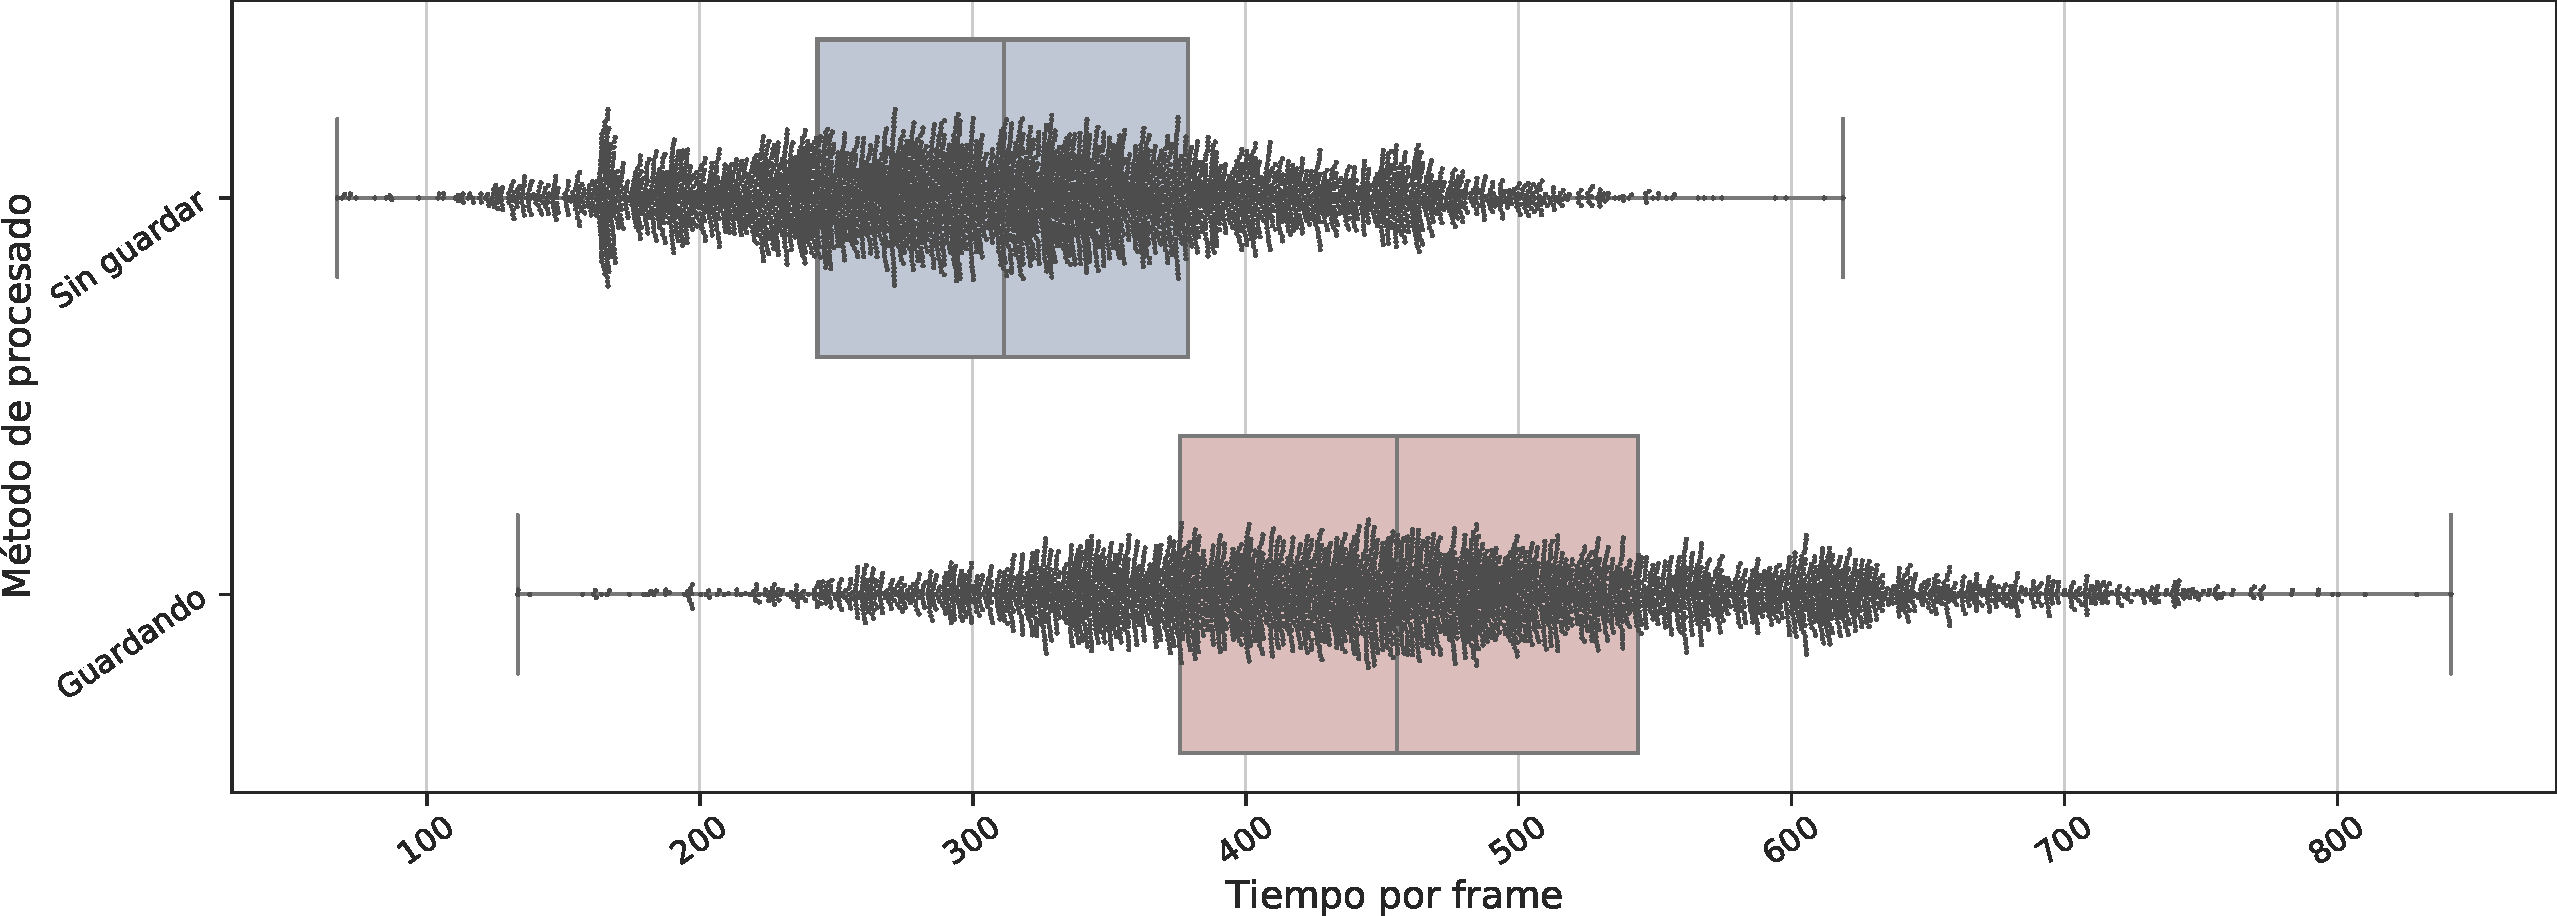
\includegraphics[width=1\textwidth]{TiemposModelo}
	\caption{Resultado ejecución de solo la posición y comparación del flujo en milisegundos.}
	\label{fig:res1}
\end{figure}

Como se puede observar en la figura~\ref{fig:res1}, existen algunos fotogramas que obtienen tiempos elevados en ambas ejecuciones. Estas situaciones se tuvieron que tener en cuenta en el cálculo del número de \textit{workers} necesarios en la paralelización del flujo. Debido a que en una situación ideal no habría apenas variación entre los tiempos de ejecución lo permitiría acortar de una manera más justa este número.

El número de \textit{workers} necesarios para ejecutar el flujo sin almacenar el procesado del esqueleto (modo 0) realizando solo las tareas de cálculo de posición y comparación de posiciones es:

\begin{equation}
\begin{split}
workers_{5FPS} = (313.50 + 94.25*2)*5/1000 = 2.51\\
workers_{15FPS} = (313.50 + 94.25*2)*15/1000 = 7.53
\end{split}
\end{equation}

Este resultado daría que como mínimo se deberían de utilizar 3 (5 \textit{fps}) y 8 (15 \textit{fps}) \textit{workers} a los que para que paliar los casos especiales, donde la duración del procesamiento es excesiva, se deberían de añadir al menos uno o dos.

Por otro lado, el número de \textit{workers} necesarios en el caso de que se quiera almacenar la imagen es:
\begin{equation}
\begin{split}
workers_{5FPS} = (463.00 + 117.58*2)*5/1000 = 3.49\\
workers_{15FPS} = (463.00 + 117.58*2)*15/1000 = 10.47
\end{split}
\end{equation}

Este resultado muestra la necesidad de tener un total de 4 (5 \textit{fps}) y 11 (15 \textit{fps}) \textit{workers}, a los que como en el caso anterior habría que sumar uno o dos más para las situaciones extraordinarias.

Para justificar la aproximación a la distribución normal para el uso de la media más dos veces la desviación ($2\sigma$), se puede observar la distribución de los tiempos en la figura~\ref{fig:dist1}. En la imagen se puede observar como, cogiendo estos valores para el cálculo del número de \textit{workers}, se está teniendo en cuenta el tiempo de prácticamente todas las ejecuciones.

\begin{figure}[h]
	\centering
	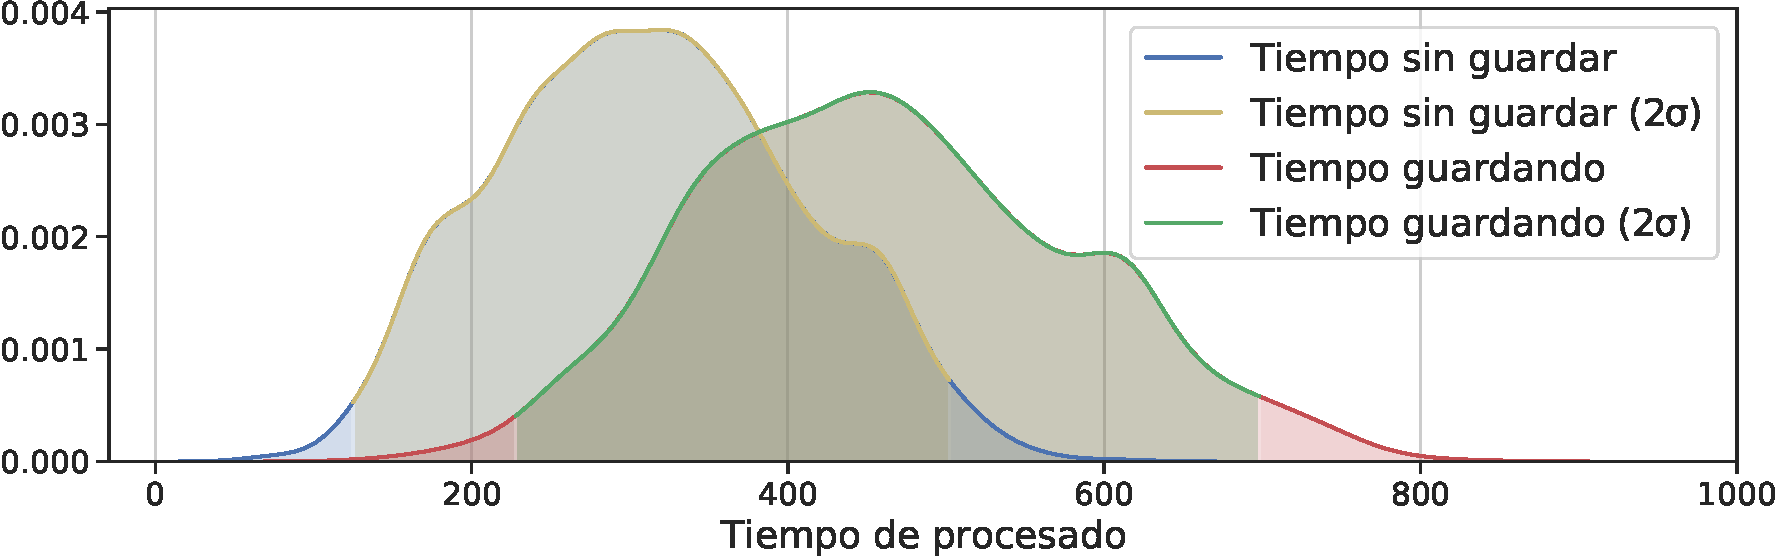
\includegraphics[width=1\textwidth]{TiemposModeloDist}
	\caption{Distribución tiempo medio de ejecución solo posición y comparación.}
	\label{fig:dist1}
\end{figure}

\subsection{Resultados flujo entero}
Los resultados obtenidos de la ejecución del flujo con todos sus componentes se pueden ver en la tabla~\ref{tab:res2}.

\begin{table}[h]
	\centering
	\resizebox{\columnwidth}{!}{
		\begin{tabular}{l|rrrrrrrr}
			\toprule
			\textbf{Tipo}&\textbf{Fotogramas}& 	\textbf{Media}& 	\textbf{Desv}& 	\textbf{Min} &	\textbf{25\%} & \textbf{50\%}&\textbf{75\%}&\textbf{Max}\\
			\midrule
			Guardando   &  $4863$ &  $626.08$&  $98.76$ & $219.33$ & $564.79$ & $636.96$ & $692.34$ & $932.61$\\
			Sin guardar &  $4863$ &  $464.04$ & $86.52$ & $193.62$ & $410.99$ & $468.62$ &  $521.74$ & $702.43$ \\
			\bottomrule
		\end{tabular}
	}
	\caption{Tabla con los resultados de la ejecución del flujo en milisegundos.}
	\label{tab:res2}
\end{table}

Como se puede observar, los tiempos medios de procesamiento de cada fotograma han aumentado unos $150$ milisegundos en el modo sin guardar y unos $200$ milisegundos en el modo con guardado añadiendo el resto del flujo. Para poder observar mejor los resultado obtenidos se realizó la gráfica que se puede ver en la figura~\ref{fig:res2}. En esta gráfica se puede ver como el tiempo medio de ejecución es de $460$ milisegundos en el modo sin guardado que es un resultado muy bueno, que como se ve a continuación necesita un número de \textit{workers} para la paralelización muy bajo.

Cabe destacar, que en el modo en el que se debería desplegar el sistema, el modo 0 sin almacenar ninguna imagen, se obtienen resultados muy destacables, siendo el máximo tiempo invertido por fotograma de poco más de $700$ milisegundos.

\begin{figure}[h]
	\centering
	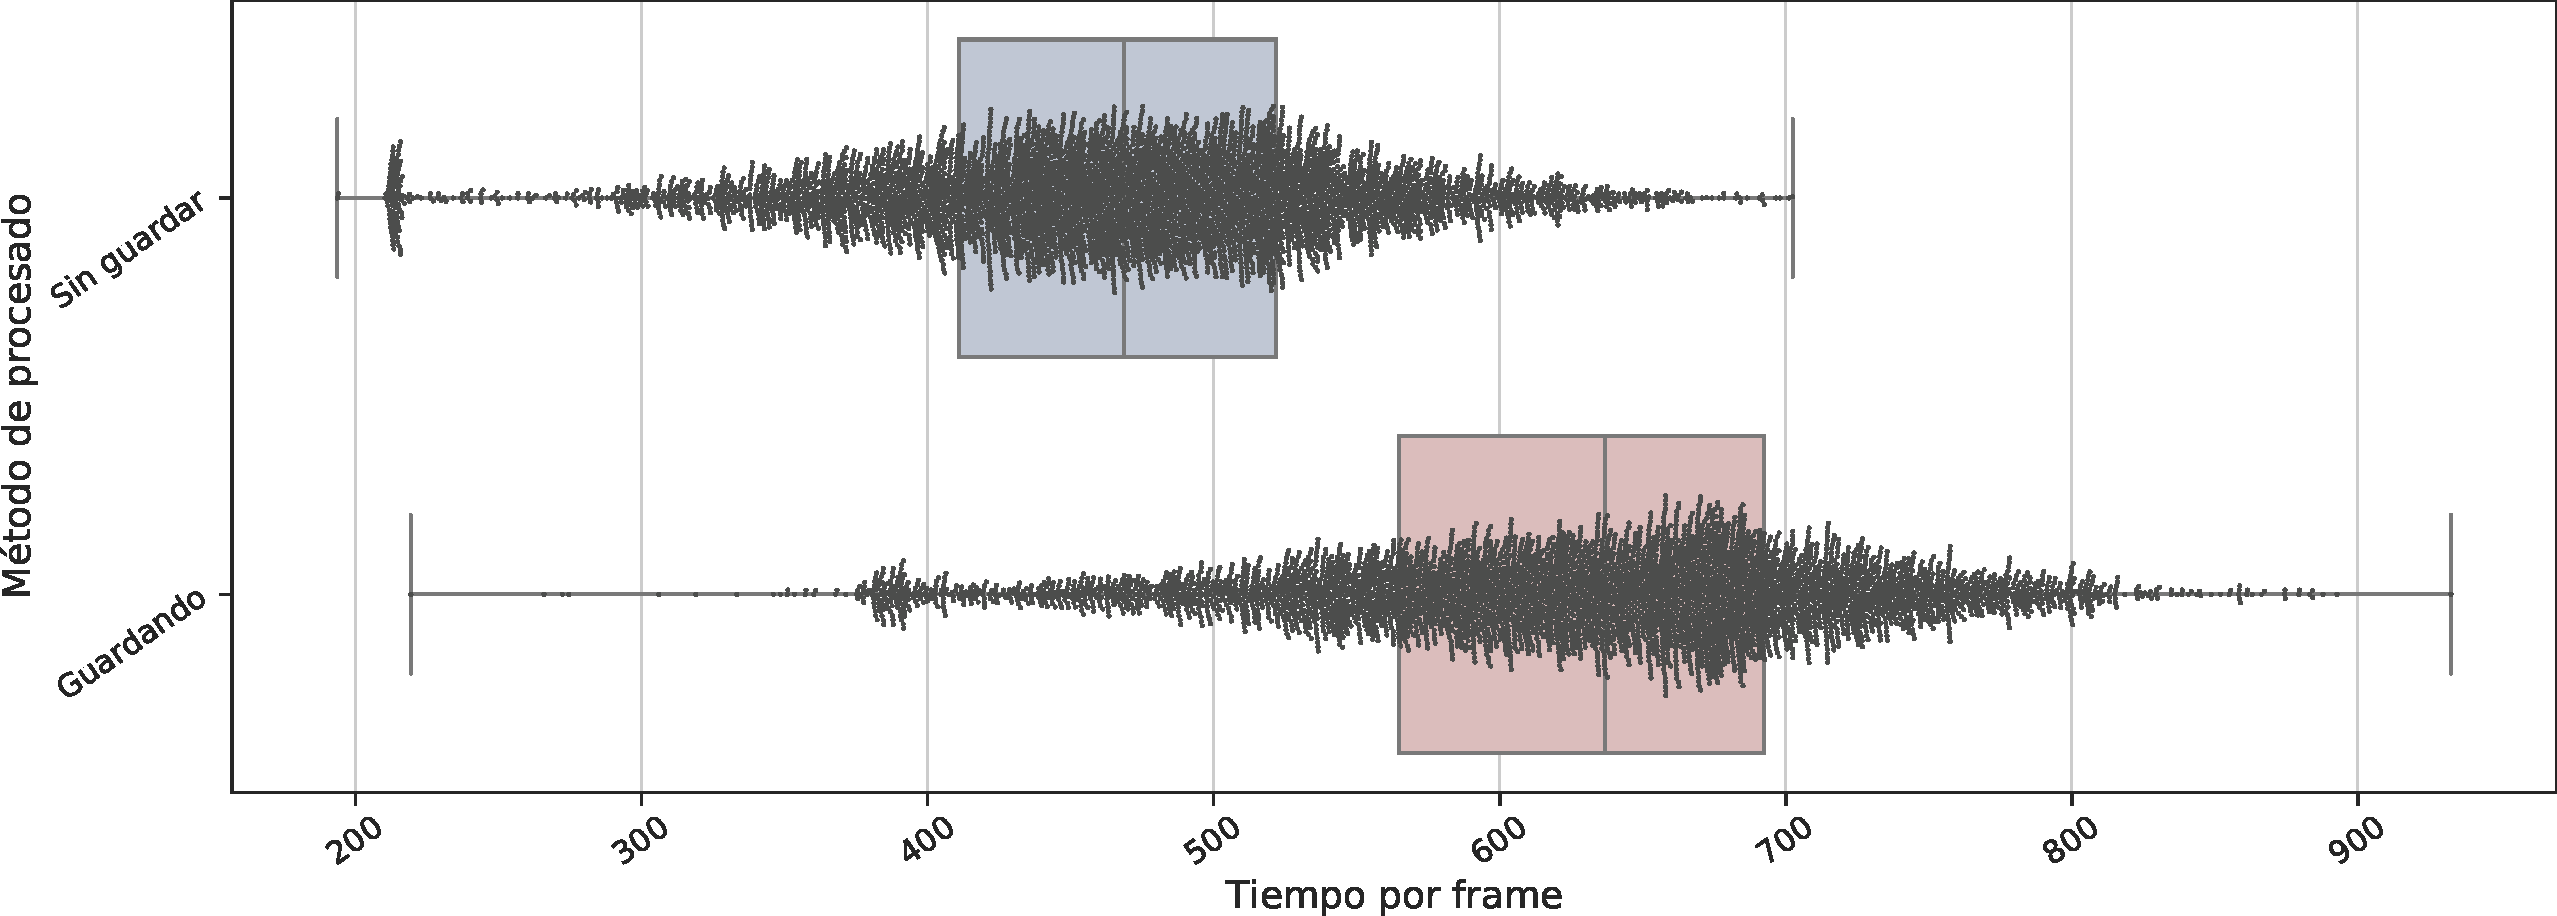
\includegraphics[width=1\textwidth]{TiemposSumados}
	\caption{Resultado ejecución flujo en milisegundos.}
	\label{fig:res2}
\end{figure}

El cálculo de los \textit{workers} necesarios para hacer el flujo paralelizable en tiempo real en el modo sin guardado se puede ver a continuación:

\begin{equation}
\begin{split}
workers_{5FPS} = (464.04 + 86.52*2)*5/1000 = 3.19\\
workers_{15FPS} = (464.04 + 86.52*2)*15/1000 = 9.56
\end{split}
\end{equation}

Con estos resultados se necesitan un total de 4 \textit{workers} en el caso de trabajar con 5 fotogramas por segundo, y de 10 \textit{workers}, como mínimo, para trabajar con vídeos de 15 fotogramas por segundos. Como en el estudio anterior, es más que recomendable añadir uno o dos \textit{workers} más a este valor para poder sobre llevar los casos extraordinarios.

Para el modo en el que se procesa y almacena la imagen se necesitan los siguientes números de \textit{workers}:
\begin{equation}
\begin{split}
workers_{5FPS} = (626.08 + 98.76*2)*5/1000 = 4.11\\
workers_{15FPS} = (626.08 + 98.76*2)*15/1000 = 12.35
\end{split}
\end{equation}

A partir de este cálculo se puede afirmar que para poder procesar un vídeo en tiempo real y obtener las imágenes resultantes se deberían de usar al menos 5 \textit{workers} en el caso de que el vídeo se retransmita a 5 fotogramas por segundos, y de 13 \textit{workers} si el vídeo es de 15 fotogramas por segundos. Como en todos los casos anteriores, se recomienda añadir al menos un \textit{worker} más para asegurar el correcto funcionamiento ante ejecuciones extraordinarias.

Como en el caso anterior, se muestra la distribución de los resultados (figura~\ref{fig:dist2}) para comprobar que con la aproximación a una distribución normal y el uso de dos veces la desviación se recogen la mayoría de los resultados.

\begin{figure}[h]
	\centering
	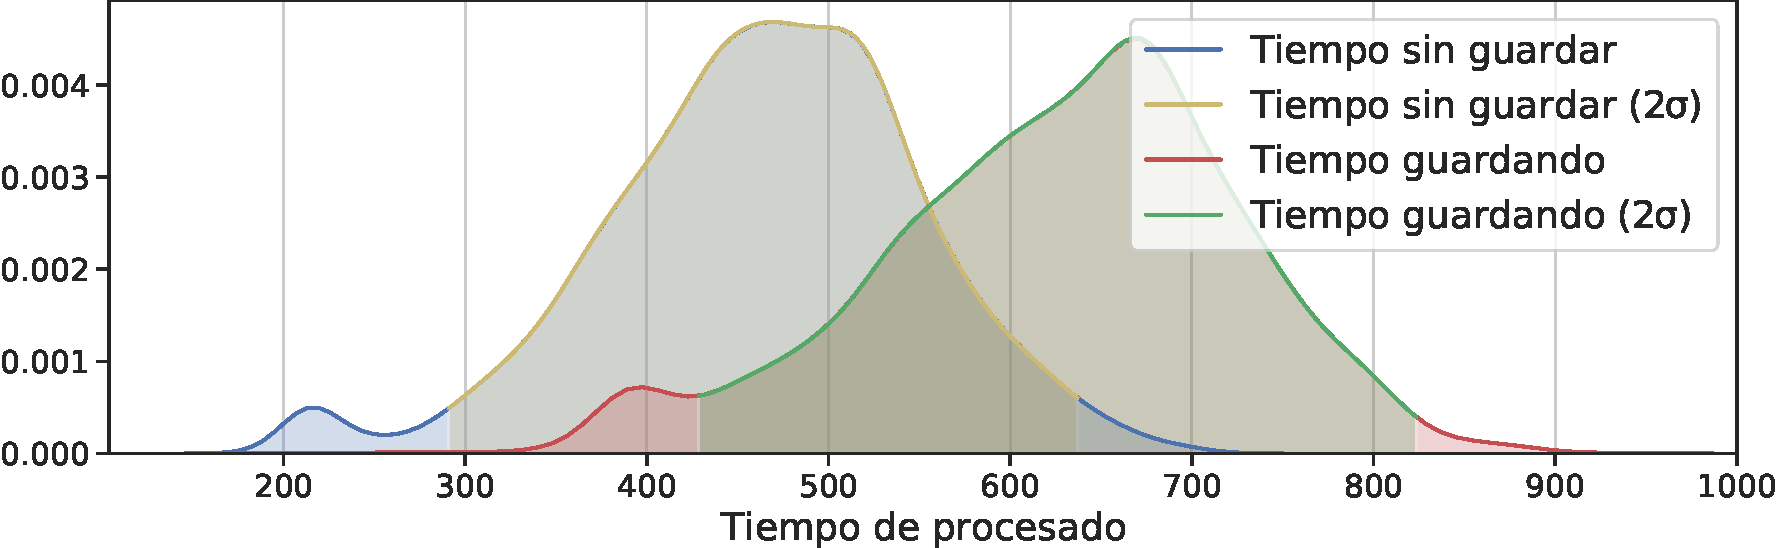
\includegraphics[width=1\textwidth]{TiemposSumadosDist}
	\caption{Distribución tiempo medio de ejecución flujo.}
	\label{fig:dist2}
\end{figure}

\section{Visualización final}
Para poder mostrar el resultado final del proyecto se implementó un \textit{Jupyter Notebook} final en donde se realiza la comparación de dos vídeos fotograma a fotograma. Con los resultados obtenidos, y los conocimientos adquiridos en el máster de distintas librerías de visualización de datos en \textit{Python} como \textit{Matplotlib} o \textit{Plotly}, se realizó una visualización de los resultados.

Esta visualización se divide en 4 partes, dependiendo a qué datos se esté centrando, ya que hay una parte que se centra en la comparación general del ejercicio, mientras que existen otros tres que se centran cada una en una zona estudiada (brazos, piernas y torso).

En cada una de las partes, como se ve en el ejemplo de la comparación general en la figura~\ref{fig:demofinal}, se realizan las siguientes visualizaciones:
\begin{itemize}
	\item Velocímetros del porcentaje de exactitud medio, máximo y mínimo. Este gráfico permite visualizar de forma rápida el nivel de exactitud del ejercicio, viendo además los valores mínimos y máximo para poder comprobar la fluctuación de la exactitud dentro de un mismo ejercicio.
	\item Evolución del porcentaje de exactitud, y comparación con la media. Este gráfico permite ver la evolución del porcentaje de exactitud a lo largo del ejercicio, lo que permite conocer qué parte del ejercicio ha sido más difícil o más sencilla para el paciente.
	\item Fotogramas que obtienen el mayor porcentaje de exactitud.
	\item Fotograma que obtiene el menor porcentaje de exactitud.
	\item Gráfico de radares, solo en la visualización general, donde se ve la relación entre las zonas en sus valores de medios, máximos y mínimos.
\end{itemize}

\begin{figure}[h]
	\centering
	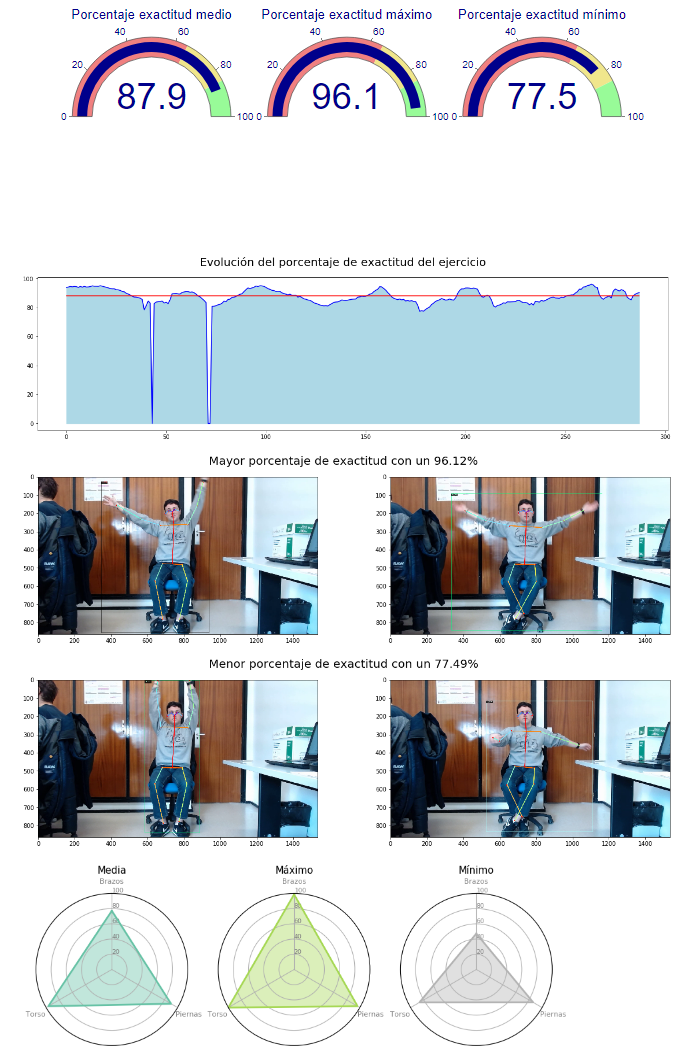
\includegraphics[width=1\textwidth]{demo}
	\caption{Ejemplos visualización final de resultados.}
	\label{fig:demofinal}
\end{figure}

Con esta visualización se ha podido mostrar un ejemplo de los gráficos que se podrán hacer en el despliegue de la herramienta. Gracias a estas visualizaciones los terapeutas podrán entender cómo ha sido la rehabilitación del paciente, sabiendo en qué partes falla más y cuales son las partes donde lo hace mejor, conocer su evolución$\ldots$ Todo ello para poder dar el mejor servicio a los pacientes. 

